\documentclass[11pt,a4paper]{article}

%% --- Geometry & spacing ------------------------------------------------
\usepackage[margin=1in,headheight=14pt]{geometry}
\usepackage{setspace}
\onehalfspacing

%% --- Encoding ----------------------------------------------------------
\usepackage[T1]{fontenc}
\usepackage[utf8]{inputenc}

%% --- Math (load before newpxmath to avoid \Bbbk / \openbox clashes) ----
\usepackage{amsmath}
\usepackage{amssymb}
\usepackage{amsthm}
\usepackage{bm}

%% --- Fonts -------------------------------------------------------------
\let\openbox\undefined
\let\Bbbk\undefined
\usepackage{newpxtext}
\usepackage{newpxmath}
\usepackage{microtype}

%% --- Tables & figures --------------------------------------------------
\usepackage{booktabs}
\usepackage{tabularx}
\usepackage{multirow}
\usepackage{array}
\usepackage{siunitx}
\sisetup{
  detect-all,
  group-digits=none,
  table-format=2.4,
  table-number-alignment=center,
}
\usepackage{graphicx}
\usepackage{caption}
\usepackage{subcaption}
\captionsetup{font=small,labelfont=bf,format=plain}
\captionsetup[sub]{font=footnotesize}

%% --- Bibliography & cross-refs -----------------------------------------
\usepackage[round,authoryear]{natbib}
\usepackage{hyperref}
\hypersetup{
  colorlinks=true,
  linkcolor=black,
  citecolor=NavyBlue,
  urlcolor=NavyBlue,
  pdfborder={0 0 0},
}
\usepackage[dvipsnames]{xcolor}

%% --- Headers / footers -------------------------------------------------
\usepackage{fancyhdr}
\pagestyle{fancy}
\fancyhf{}
\fancyhead[L]{\small \textsc{Backtesting Expected Shortfall}}
\fancyhead[R]{\small \thepage}
\renewcommand{\headrulewidth}{0pt}

%% --- Title block ------------------------------------------------------
\usepackage{titlesec}
\titleformat{\section}{\normalfont\Large\bfseries\color{black!85}}{\thesection}{0.7em}{}
\titleformat{\subsection}{\normalfont\large\bfseries\color{black!75}}{\thesubsection}{0.7em}{}
\titleformat{\subsubsection}{\normalfont\normalsize\bfseries\itshape}{\thesubsubsection}{0.7em}{}

%% --- Macros ------------------------------------------------------------
\newcommand{\VaR}{\operatorname{VaR}}
\newcommand{\ES}{\operatorname{ES}}
\newcommand{\R}{\mathbb{R}}
\newcommand{\E}{\mathbb{E}}
\newcommand{\Var}{\operatorname{Var}}
\newcommand{\Cov}{\operatorname{Cov}}
\newcommand{\Prob}{\mathbb{P}}
\newcommand{\one}{\mathbf{1}}
\newcommand{\given}{\,|\,}
\newcommand{\code}[1]{\texttt{\small #1}}
\newcommand{\package}[1]{\texttt{#1}}

\theoremstyle{plain}
\newtheorem{prop}{Proposition}

%% =====================================================================
\title{
  \vspace{-2em}
  \Large \textsc{Backtesting Expected Shortfall:} \\[0.2em]
  \LARGE A Battery of Eleven Statistics \\
  Across Five Equity Indices and Five Crisis Windows
}
\author{Dan Allouche}
\date{May 2026}

%% =====================================================================
\begin{document}
\maketitle

\begin{abstract}
\noindent
This paper implements eleven expected-shortfall (ES) and value-at-risk
(VaR) backtests on a common out-of-sample slice and reports their
joint behaviour on real and simulated data. The battery covers the
basic and robust statistics of \citet{du_escanciano_2017}, the
parametric Monte-Carlo $Z_1$ and $Z_2$ checks of
\citet{acerbi_szekely_2014}, the multinomial VaR test of
\citet{kratz_lok_mcneil_2018}, the conditional-coverage decomposition
of \citet{christoffersen_1998}, the proportion-of-failures test of
\citet{kupiec_1995}, and the standardised-exceedance bootstrap of
\citet{mcneil_frey_2000}. On the S\&P 500 the eleven tests give
inconsistent verdicts: nine reject on the Global Financial Crisis
window, ten on the COVID-19 window, and the three tests that fail to
reject (Christoffersen independence, Acerbi--Szekely $Z_1$,
McNeil--Frey) do so on both crises. The same pattern holds across a
grid of five equity indices and five crisis windows: the unconditional
block ($U_{ES}$, $U_{VaR}$, Kupiec, multinomial, $Z_2$) rejects in
$19$--$20$ of $20$ non-SVB cells, while the day-to-day independence
component rejects only $2$ of $20$. A Monte Carlo size-and-power study
on $16{,}000$ simulated paths shows that the marginal-coverage tests
over-reject at $n=1000$ (empirical size up to $16\%$) and that, under
strong asymmetric leverage, $Z_2$ rejects almost twice as often as
$Z_1$ ($0.23$ versus $0.12$). An LSTM-Quantile baseline trained on
$2010$--$2019$ fails to scale during the March 2020 spike, under-calling
VaR by a factor of $2.6$ relative to AR(1)-GARCH(1,1)-$t$ and rejecting
the Kupiec test with a statistic almost twenty times the GARCH value;
a mixture-density extension of the same LSTM backbone supplies the
analytic CDF the LSTM-Quantile lacks and unlocks the full battery on
the neural baseline, reducing the under-call factor from $2.6$ to
$1.3$. A separate four-variant comparison shows that switching the
GARCH(1,1) leverage term flips the verdict on five of the eleven
tests on the same OOS data. The paper concludes that ES should not
be backtested by a single statistic, and that the choice of
forecasting model is part of the backtest, not a separable input.
\end{abstract}

\thispagestyle{empty}
\newpage
\pagenumbering{roman}
\setcounter{page}{2}

\tableofcontents
\clearpage
\pagenumbering{arabic}
\setcounter{page}{1}

%% =====================================================================
\section{Introduction}
\label{sec:intro}

The Fundamental Review of the Trading Book \citep{bcbs_2019} replaced
value-at-risk with expected shortfall as the primary market-risk
measure for regulatory capital. VaR at level $\alpha$ is the
$(1-\alpha)$-quantile of the loss distribution; ES at the same level
is the average loss conditional on being beyond the VaR. ES corrects
the two well-known shortcomings of VaR: it is sub-additive, hence a
coherent risk measure in the sense of \citet{artzner_etal_1999}, and
it accounts for the magnitude of the losses in the tail rather than
their mere frequency.

The transition exposes a tension. VaR admits a simple backtest based
on counting violation days, codified in \citet{kupiec_1995} and refined
into a conditional-coverage decomposition by \citet{christoffersen_1998}.
ES does not: \citet{gneiting_2011} shows that ES is not
\emph{elicitable} as a single functional, which rules out a strictly
proper scoring rule of the kind that exists for VaR (the pinball
loss). The literature has responded with a dozen alternative test
statistics, each making different assumptions on the data-generating
process, on parameter-estimation uncertainty, and on the joint
elicitation of $(\VaR, \ES)$ \citep{fissler_ziegel_2016,
nolde_ziegel_2017}. Practitioners typically pick one and ship it. The
question this paper takes seriously is whether that choice
is benign.

\paragraph{Contributions.} The paper makes five contributions. First,
it implements eleven of the leading ES and VaR backtests in a single
unified battery and reports them on the same out-of-sample slice. The
battery covers the four basic and the two robust statistics of
\citet{du_escanciano_2017}; the parametric Monte-Carlo $Z_1$ and $Z_2$
of \citet{acerbi_szekely_2014}; the multinomial test of
\citet{kratz_lok_mcneil_2018}; the proportion-of-failures test of
\citet{kupiec_1995} and the conditional-coverage decomposition of
\citet{christoffersen_1998}; and the standardised-exceedance bootstrap
of \citet{mcneil_frey_2000}. Second, it runs the battery on a grid of
five equity indices (S\&P~500, Nasdaq~100, FTSE~100, DAX, Nikkei~225)
and five crisis windows (Dotcom, the Global Financial Crisis,
COVID-19, the 2022 inflation shock, and the March 2023 banking shock)
under a common AR(1)-GARCH(1,1)-$t$ forecasting model, producing $275$
p-values. Third, it quantifies the finite-sample size and power of
the battery on simulated paths drawn from a correctly-specified DGP
and from three alternative DGPs with asymmetric leverage and Gaussian
tails. Fourth, it isolates the forecasting-model contribution by
running the eleven base tests on the four
$(\text{vol},\text{dist}) \in \{\text{GARCH},\text{GJR}\} \times
\{t, \mathcal{N}\}$ combinations on the same OOS window, showing
that the GARCH-variant choice flips five of the eleven verdicts.
Fifth, it extends the LSTM-Quantile baseline into a mixture-density
network whose parametric output unlocks the full battery on the
neural model.

\paragraph{Roadmap.} Section~\ref{sec:method} fixes notation and
presents the eleven backtests with their asymptotic null distributions.
Section~\ref{sec:data} describes the data and the crisis windows.
Section~\ref{sec:results} reports the empirical results.
Section~\ref{sec:discussion} discusses what the battery says about the
choice of a single test in operational use. Section~\ref{sec:conclusion}
concludes. Two appendices document the software architecture and the
exact recipe to reproduce every number in the paper.

%% =====================================================================
\section{Methodology}
\label{sec:method}

Let $Y_t$ denote the percentage log-return at date $t$, with the sign
convention that a loss is $-Y_t > 0$. Let $\mathcal{F}_{t-1}$ denote
the information set available through $t-1$, and let $F_t$ be the
one-step-ahead conditional distribution of $Y_t$ given
$\mathcal{F}_{t-1}$. Value-at-risk and expected shortfall at level
$\alpha \in (0,1)$ are defined by
\begin{equation}
  \VaR_t(\alpha) = -F_t^{-1}(\alpha),
  \qquad
  \ES_t(\alpha) = \frac{1}{\alpha} \int_0^\alpha \VaR_t(u)\, du.
  \label{eq:var-es-def}
\end{equation}
Under correct conditional specification $\Prob(-Y_t > \VaR_t(\alpha)
\given \mathcal{F}_{t-1}) = \alpha$, and ES is the conditional mean of
$-Y_t$ given $-Y_t > \VaR_t(\alpha)$.

\subsection{PIT residuals and violation indicators}
\label{sec:method-pit}

The \emph{probability integral transform} of $Y_t$ under $F_t$ is
\begin{equation}
  u_t = F_t(Y_t).
  \label{eq:pit}
\end{equation}
Under correct conditional specification $\{u_t\}$ is i.i.d.\ uniform
on $[0,1]$, which is the substrate the
\citet{du_escanciano_2017} battery exploits. Two derived series carry
the test signal:
\begin{align}
  h_t(\alpha) &= \one\{u_t \leq \alpha\}, \\
  H_t(\alpha) &= \frac{1}{\alpha}\,(\alpha - u_t)\, \one\{u_t \leq \alpha\}.
  \label{eq:h-H}
\end{align}
$h_t$ is the binary VaR violation indicator; $H_t$ is its continuous
counterpart, equal to zero on a non-violation day and growing linearly
with how far in the tail the loss lies on a violation day. Under
correct specification,
\begin{equation}
  \E[h_t] = \alpha,
  \quad \Var(h_t) = \alpha(1-\alpha),
  \quad \E[H_t] = \frac{\alpha}{2},
  \quad \Var(H_t) = \alpha\!\left(\tfrac{1}{3} - \tfrac{\alpha}{4}\right).
  \label{eq:moments}
\end{equation}

\paragraph{Two conventions.} \citet{du_escanciano_2017} report ES at
$\alpha_{ES} = 2\,\alpha_{VaR}$ (e.g.\ $0.10$ and $0.05$); the
Basel III standard \citep{bcbs_2019} sets $\alpha_{VaR} = 0.025$ and
keeps the same level for ES. The \citet{acerbi_szekely_2014} and
\citet{mcneil_frey_2000} statistics assume
$\alpha_{ES} = \alpha_{VaR}$ because both reference the same set of
VaR exceptions. The implementation keeps both conventions in scope:
the Du--Escanciano block runs at the paper's
$\alpha_{ES} = 2\,\alpha_{VaR}$, and the Acerbi--Szekely / McNeil--Frey
block re-evaluates the VaR and ES paths at $\alpha_{VaR}$ before
running the test, so the legend of every result table reports the
exact level used.

\subsection{Eleven backtests}
\label{sec:method-battery}

The eleven backtests split into three groups. Group~A
(Du--Escanciano) operates on $u_t$, $h_t$ and $H_t$. Group~B (VaR
baselines) operates on $h_t$ only. Group~C (ES baselines) operates on
the realised losses, the VaR path, the ES path, and the conditional
volatility. Table~\ref{tab:battery} summarises the asymptotic null
distributions. The two robust Du--Escanciano variants ($MU_{ES}$ and
$MC_{ES}$) require the fitted parameter vector, the in-sample window,
and the realised series, so they augment the four basic statistics
when those inputs are available.

\subsubsection*{Group A: Du--Escanciano (2017)}

The unconditional ES statistic is
\begin{equation}
  U_{ES} = \frac{\sqrt{n}\,\bigl(\bar{H} - \alpha/2\bigr)}{\sqrt{\alpha\,(1/3 - \alpha/4)}},
  \qquad \bar{H} = \frac{1}{n}\sum_{t=1}^n H_t(\alpha),
  \label{eq:U_ES}
\end{equation}
asymptotically $\mathcal{N}(0,1)$ under correct specification. The
conditional ES Box--Pierce statistic stacks the first $m$ sample
autocorrelations $\hat{\rho}_j$ of $H_t - \alpha/2$:
\begin{equation}
  C_{ES}(m) = n \sum_{j=1}^{m} \hat{\rho}_j^2,
  \label{eq:C_ES}
\end{equation}
asymptotically $\chi^2(m)$. $U_{VaR}$ and $C_{VaR}(m)$ are defined
identically with $h_t - \alpha$ in place of $H_t - \alpha/2$.

The robust variants correct the variance of the test statistic for
parameter-estimation uncertainty. Let $\hat{\bm\theta}$ denote the
maximum-likelihood estimator on an in-sample window of length $T$ and
let $\hat{W} = T \cdot \widehat{\Cov}(\hat{\bm\theta})$. With
\begin{equation}
  \bm R_{ES} \;=\; \frac{\partial \bar{H}}{\partial \bm\theta}\bigg|_{\hat{\bm\theta}}
  \label{eq:R_ES}
\end{equation}
obtained by central differences (step
$\max(|\hat\theta_k|\,\varepsilon_{\text{rel}}, \varepsilon_{\text{min}})$
with $\varepsilon_{\text{rel}}=10^{-5}$ and
$\varepsilon_{\text{min}}=10^{-7}$), the robust unconditional ES
statistic is
\begin{equation}
  MU_{ES} \;=\; \frac{\sqrt{n}\,\bigl(\bar{H} - \alpha/2\bigr)}{\sqrt{\alpha\,(1/3-\alpha/4) + (n/T)\,\bm R_{ES}^\top \hat{W} \bm R_{ES}}}.
  \label{eq:MU_ES}
\end{equation}
$MC_{ES}(m)$ is the analogous correction of $C_{ES}(m)$.

\subsubsection*{Group B: VaR baselines}

Let $N = \sum_t h_t(\alpha)$ be the realised number of violations.
The Kupiec proportion-of-failures statistic is
\begin{equation}
  \mathrm{LR}_{POF}
  \;=\; -2 \log \!\left[
    \frac{\alpha^N (1-\alpha)^{n-N}}{\hat\pi^N (1-\hat\pi)^{n-N}}
  \right],
  \qquad \hat\pi = N/n,
  \label{eq:kupiec}
\end{equation}
asymptotically $\chi^2(1)$. The \citet{christoffersen_1998}
decomposition adds an independence component
$\mathrm{LR}_{IND}$ from a two-state Markov chain on
$\{h_t\}$ (also $\chi^2(1)$) and a joint conditional-coverage
component
\begin{equation}
  \mathrm{LR}_{CC} = \mathrm{LR}_{POF} + \mathrm{LR}_{IND} \sim \chi^2(2).
  \label{eq:LR_CC}
\end{equation}
The decomposition is exact, so a rejection of $\mathrm{LR}_{CC}$
combined with a non-rejection of $\mathrm{LR}_{IND}$ identifies the
coverage component as the source.

The \citet{kratz_lok_mcneil_2018} multinomial test takes a vector of
$K$ VaR levels $(\alpha_1 < \dots < \alpha_K)$ and tests jointly
whether the observed counts in the $K+1$ bins of the empirical
distribution match the multinomial model implied by the conditional
distribution. The implementation uses $K=4$ at
$\alpha \in \{0.025,\,0.05,\,0.075,\,0.10\}$; the asymptotic null is
$\chi^2(K)$.

\subsubsection*{Group C: ES baselines}

The \citet{acerbi_szekely_2014} $Z_1$ and $Z_2$ statistics compare
realised losses to the conditional ES:
\begin{align}
  Z_1 &= \frac{1}{N}\sum_{t: -Y_t > \VaR_t}\!\!\frac{-Y_t}{\ES_t} \;-\; 1, \\
  Z_2 &= \sum_{t=1}^n \frac{(-Y_t)\,\one\{-Y_t > \VaR_t\}}{n\,\alpha\,\ES_t} \;-\; 1.
  \label{eq:Z1-Z2}
\end{align}
$Z_1$ averages the loss-to-ES ratio over the empirical violation set;
$Z_2$ aggregates over the full window. Both have $\E[Z] = 0$ under
correct ES specification. The implementation draws $n_{\text{sim}}$
paths from the fitted AR(1)-GARCH(1,1)-$t$ at the same conditional
moments, replaces the realised innovations with fresh i.i.d.\
standardised-$t$ draws, and reads the upper-tail Monte-Carlo p-value.
$n_{\text{sim}} = 10{,}000$ in the CLI runs and $2{,}000$ in the
Monte-Carlo size-and-power study.

The \citet{mcneil_frey_2000} statistic forms the standardised
exceedances
\begin{equation}
  r_t \;=\; \frac{-Y_t - \ES_t}{\sigma_t}
  \quad \text{for } t \text{ with a VaR violation},
  \label{eq:mcneil-frey}
\end{equation}
and tests $\E[r_t \given -Y_t > \VaR_t] = 0$ against a stationary block
bootstrap distribution. Under correct ES specification at the same
level as the VaR, the residual of the realised loss against the
conditional ES averages to zero on the violation set, since ES is
precisely the conditional mean of the loss given a violation. The
CLI default is $n_{\text{boot}} = 10{,}000$.

\begin{table}[ht]
\centering
\caption{The eleven-test battery. The robust statistics
$MU_{ES}$ and $MC_{ES}$ require the fitted parameter vector and
the in-sample window; the basic battery runs without them.}
\label{tab:battery}
\small
\begin{tabular}{@{}llll@{}}
\toprule
\textbf{Test} & \textbf{Targets} & \textbf{Asymptotic null} & \textbf{Reference} \\
\midrule
$U_{ES}$              & ES unconditional             & $\mathcal{N}(0,1)$ & \citealt{du_escanciano_2017} \\
$C_{ES}(m)$           & ES conditional (Box--Pierce) & $\chi^2(m)$        & \citealt{du_escanciano_2017} \\
$MU_{ES}$             & ES unconditional, robust     & $\mathcal{N}(0,1)$ & \citealt{du_escanciano_2017} \\
$MC_{ES}(m)$          & ES conditional, robust       & $\chi^2(m)$        & \citealt{du_escanciano_2017} \\
$U_{VaR}$             & VaR unconditional            & $\mathcal{N}(0,1)$ & \citealt{du_escanciano_2017} \\
$C_{VaR}(m)$          & VaR conditional              & $\chi^2(m)$        & \citealt{du_escanciano_2017} \\
$\mathrm{Kupiec}_{POF}$       & VaR proportion-of-failures   & $\chi^2(1)$        & \citealt{kupiec_1995} \\
$\mathrm{Christoffersen}_{CCI}$ & VaR independence             & $\chi^2(1)$        & \citealt{christoffersen_1998} \\
$\mathrm{Christoffersen}_{CC}$  & VaR coverage + independence  & $\chi^2(2)$        & \citealt{christoffersen_1998} \\
$\mathrm{KLM}_{\text{mult}}(K)$ & ES via multi-level VaR       & $\chi^2(K)$        & \citealt{kratz_lok_mcneil_2018} \\
$Z_1$, $Z_2$          & ES (parametric Monte Carlo)  & simulated          & \citealt{acerbi_szekely_2014} \\
$\mathrm{McNeil}\text{--}\mathrm{Frey}$ & ES via standardised exceedances & bootstrap & \citealt{mcneil_frey_2000} \\
\bottomrule
\end{tabular}
\end{table}

\subsection{Forecasting model}
\label{sec:method-model}

The baseline conditional model is AR(1)-GARCH(1,1) with standardised
Student-$t$ innovations:
\begin{align}
  Y_t       &= c + \phi\,Y_{t-1} + \varepsilon_t, \\
  \varepsilon_t &= \sigma_t\,z_t, \\
  \sigma_t^2 &= \omega + \alpha_1\,\varepsilon_{t-1}^2 + \beta_1\,\sigma_{t-1}^2, \\
  z_t       &\overset{\text{i.i.d.}}{\sim} t_\nu \text{ standardised to unit variance.}
  \label{eq:garch}
\end{align}
The parameters $(c, \phi, \omega, \alpha_1, \beta_1, \nu)$ are
estimated by conditional maximum likelihood using the \package{arch}
package \citep{engle_1982,bollerslev_1986}. The recursion is run on
the full history so the out-of-sample residuals are conditioned on the
in-sample-fitted dynamics rolling forward without re-estimation; the
recursion clips $\sigma_t^2$ to be non-negative before the square
root to absorb numerical noise from ill-conditioned MLE fits on very
short windows.

Two variants extend the baseline: the GJR-GARCH(1,1,1) of
\citet{glosten_jagannathan_runkle_1993},
\begin{equation}
  \sigma_t^2 = \omega + \bigl(\alpha_1 + \gamma\,\one\{\varepsilon_{t-1} < 0\}\bigr)\varepsilon_{t-1}^2 + \beta_1\,\sigma_{t-1}^2,
  \label{eq:gjr}
\end{equation}
which adds the asymmetric leverage term $\gamma$, and a Gaussian
innovation flavour where $z_t \sim \mathcal{N}(0,1)$. The four
combinations $(\mathrm{GARCH},t), (\mathrm{GARCH}, \mathcal{N}),
(\mathrm{GJR},t), (\mathrm{GJR},\mathcal{N})$ share a single recursion
helper with $\gamma=0$ recovering the symmetric case.

Two neural baselines are included for contrast. The first is the
\emph{LSTM-Quantile} head of \citet{hochreiter_schmidhuber_1997},
which maps a length-$L$ window of past returns to two outputs
$(\hat{\VaR}_t, \hat{\ES}_t)$ through a stacked LSTM whose hidden
state feeds two linear heads. The ES head is parameterised as
$\hat\ES_t = \hat\VaR_t + \mathrm{softplus}(\cdot)$, so $\hat\ES_t
\geq \hat\VaR_t$ holds by construction. The training loss is the
pinball loss for VaR plus the FZ0 loss of \citet{fissler_ziegel_2016}
for the joint $(\VaR, \ES)$ pair. The LSTM-Quantile has no
closed-form PIT and so receives only the subset of the battery that
does not require $u_t$.

The second is the \emph{mixture-density LSTM} (MDN-LSTM), which
shares the same LSTM backbone but replaces the two-output head with
three linear heads that parameterise the conditional Student-$t$ on
the next return: $Y_{t+1} \sim t_{\nu_t}(\mu_t, \sigma_t)$. The
scale $\sigma_t$ is positivity-constrained via softplus and the
degrees of freedom $\nu_t$ are constrained above two (so the
variance is finite) via $\mathrm{softplus}(\cdot) + 2$. The training
loss is the negative log-likelihood of the predicted distribution,
which is a strictly proper scoring rule. Because the MDN supplies a
closed-form CDF, every quantity the battery needs follows in closed
form: the PIT residual
$u_t = \mathrm{cdf}_{t_{\nu_t}}(Y_t \mid \mu_t, \sigma_t)$, the
analytic VaR and ES, and a per-day Student-$t$ simulator for the
Acerbi--Szekely Monte-Carlo p-values. Eleven of the thirteen battery
statistics therefore apply on the MDN-LSTM; the two robust
Du--Escanciano variants $MU_{ES}$ and $MC_{ES}$ remain unreachable
because they require the parameter covariance of an MLE fit, which
the stochastic-gradient-trained network does not expose in closed
form.

%% =====================================================================
\section{Data}
\label{sec:data}

The data are end-of-day adjusted closing prices for five equity
indices, downloaded from Yahoo Finance and converted to log-returns in
percent. Table~\ref{tab:data} lists the tickers and the in-sample and
out-of-sample windows. The full S\&P~500 sample covers $7{,}044$
trading days from January 1997 to December 2024 and is pinned to a
frozen parquet file under \code{tests/data/} so back-fills by the
upstream vendor cannot alter the reference numbers in this paper.

\begin{table}[ht]
\centering
\caption{Equity indices and crisis windows. Each (asset, crisis) cell
uses a five-year in-sample window ending the day before the crisis
out-of-sample slice.}
\label{tab:data}
\small
\begin{tabular}{@{}llcc@{}}
\toprule
\textbf{Crisis} & \textbf{Out-of-sample window} & \textbf{Trading days} & \textbf{In-sample window} \\
\midrule
Dotcom              & 2000-04-01 \,--\, 2002-12-31 & 689 & 1995-04-01 \,--\, 2000-03-31 \\
Global Financial Crisis & 2007-07-01 \,--\, 2009-06-30 & 504 & 2002-07-01 \,--\, 2007-06-30 \\
COVID-19            & 2020-01-01 \,--\, 2021-12-31 & 505 & 2015-01-01 \,--\, 2019-12-31 \\
Inflation 2022      & 2022-01-01 \,--\, 2022-12-31 & 251 & 2017-01-01 \,--\, 2021-12-31 \\
SVB / regional banks & 2023-03-01 \,--\, 2023-09-30 & 148 & 2018-03-01 \,--\, 2023-02-28 \\
\bottomrule
\end{tabular}
\smallskip

\begin{tabular}{@{}lll@{}}
\toprule
\textbf{Asset} & \textbf{Ticker} & \textbf{Market} \\
\midrule
S\&P 500            & \code{\^{}GSPC}   & US large cap \\
Nasdaq 100          & \code{\^{}NDX}    & US tech \\
FTSE 100            & \code{\^{}FTSE}   & UK large cap \\
DAX                 & \code{\^{}GDAXI}  & German large cap \\
Nikkei 225          & \code{\^{}N225}   & Japan large cap \\
\bottomrule
\end{tabular}
\end{table}

The single-asset replication in Section~\ref{sec:res-single} uses the
S\&P 500 over two of these crises (GFC and COVID-19), with the
in-sample windows from \citet{du_escanciano_2017} extended by one
decade. The multi-asset grid in Section~\ref{sec:res-grid} uses all
five (asset, crisis) combinations on the same five-year-in-sample
template.

%% =====================================================================
\section{Empirical results}
\label{sec:results}

\subsection{Single-asset replication: S\&P 500, GFC and COVID-19}
\label{sec:res-single}

\paragraph{Setup.} Risk levels follow the \citet{du_escanciano_2017}
convention: $\alpha_{VaR} = 0.05$, $\alpha_{ES} = 0.10$, Box--Pierce
lag $m = 5$. Two periods are reported: the Global Financial Crisis
with an in-sample window covering 1997-01-01 to 2007-06-30 ($T = 2{,}640$
days) and an OOS slice of $n = 504$ days from 2007-07-01 to 2009-06-30;
and the COVID-19 crash with in-sample 2010-01-01 to 2019-12-31
($T \approx 2{,}516$ days) and OOS $n = 505$ days from 2020-01-01 to
2021-12-31. The AR(1)-GARCH(1,1)-$t$ fit gives
$\hat\nu = 8.72$ on the GFC in-sample window and $\hat\nu = 4.83$ on the
COVID in-sample window. The 2010--2019 in-sample tail is empirically
fatter than the 1997--2007 in-sample tail; neither training window
contains the March 2020 shock, which lies entirely in the COVID OOS
slice. Realised VaR violations are $44$ out of $504$ on the GFC OOS
slice and $40$ out of $505$ on the COVID OOS slice; both exceed the
$5\%$ nominal rate of $25$ violations.

\paragraph{Battery results.} Table~\ref{tab:single} reports the full
battery on both windows: the eleven base tests plus the two robust
Du--Escanciano variants $MU_{ES}$ and $MC_{ES}$, for a total of
thirteen statistics per period. Nine tests reject at the
$5\%$ level on the GFC window; ten reject on COVID-19. The four
tests that fail to reject on at least one of the two crises are
$C_{VaR}(5)$ on GFC ($p = 0.0894$), $\mathrm{Christoffersen}_{CCI}$
on both ($p = 0.0645$ on GFC, $0.2979$ on COVID), $Z_1$ on both
($p = 0.2168$ on GFC, $0.1021$ on COVID), and McNeil--Frey on both
($p = 0.2759$ on GFC, $0.1721$ on COVID).

\begin{table}[ht]
\centering
\caption{Single-asset battery: thirteen statistics on the S\&P 500
over the Global Financial Crisis (in-sample 1997--2007, OOS
2007-07 to 2009-06) and COVID-19 (in-sample 2010--2019, OOS
2020-01 to 2021-12). Rejection at $5\%$ in bold.}
\label{tab:single}
\small
\setlength{\tabcolsep}{6pt}
\begin{tabular}{@{}l*{4}{S[table-format=2.4]}cc@{}}
\toprule
& \multicolumn{2}{c}{\textbf{GFC 2008}} & \multicolumn{2}{c}{\textbf{COVID-19}} & \multicolumn{2}{c}{\textbf{Decision}} \\
\cmidrule(lr){2-3}\cmidrule(lr){4-5}\cmidrule(lr){6-7}
\textbf{Test} & {Statistic} & {p-value} & {Statistic} & {p-value} & {GFC} & {COVID} \\
\midrule
$U_{ES}$              & 4.1968  & 0.0000 & 2.3129  & 0.0207 & \textbf{R} & \textbf{R} \\
$C_{ES}(5)$           & 14.9532 & 0.0106 & 13.8442 & 0.0166 & \textbf{R} & \textbf{R} \\
$U_{VaR}$             & 3.8423  & 0.0001 & 3.0116  & 0.0026 & \textbf{R} & \textbf{R} \\
$C_{VaR}(5)$          & 9.5390  & 0.0894 & 17.0723 & 0.0044 &           F & \textbf{R} \\
$MU_{ES}$             & 3.7395  & 0.0002 & 2.2049  & 0.0275 & \textbf{R} & \textbf{R} \\
$MC_{ES}(5)$          & 14.8936 & 0.0108 & 12.6821 & 0.0265 & \textbf{R} & \textbf{R} \\
$\mathrm{Kupiec}_{POF}$       & 12.1945 & 0.0005 & 7.7625  & 0.0053 & \textbf{R} & \textbf{R} \\
$\mathrm{Christoffersen}_{CCI}$ & 3.4167 & 0.0645 & 1.0836 & 0.2979 &           F &           F \\
$\mathrm{Christoffersen}_{CC}$  & 15.6112 & 0.0004 & 8.8461 & 0.0120 & \textbf{R} & \textbf{R} \\
$\mathrm{KLM}_{\text{mult}}(4)$ & 23.3104 & 0.0001 & 13.5039 & 0.0091 & \textbf{R} & \textbf{R} \\
$Z_1$                 & 0.0380  & 0.2168 & 0.0991 & 0.1021 &           F &           F \\
$Z_2$                 & 0.8124  & 0.0002 & 0.7412 & 0.0004 & \textbf{R} & \textbf{R} \\
$\mathrm{McNeil}\text{--}\mathrm{Frey}$ & 1.0796 & 0.2759 & 1.3609 & 0.1721 &           F &           F \\
\midrule
\multicolumn{5}{r}{\textbf{Rejections at 5\%}} & 9/13 & 10/13 \\
\bottomrule
\end{tabular}
\end{table}

The marginal-coverage block ($U_{ES}$, $U_{VaR}$, $\mathrm{Kupiec}_{POF}$,
$\mathrm{KLM}_{\text{mult}}(4)$) and the conditional-coverage block
($C_{ES}(5)$, $MU_{ES}$, $MC_{ES}(5)$, plus $C_{VaR}(5)$ on COVID)
fire on both crises. The day-to-day independence test
$\mathrm{Christoffersen}_{CCI}$ and the empirical-violation-set
statistics $Z_1$ and McNeil--Frey do not. The asymmetry is operational:
the model over-violates on aggregate but does not concentrate the
excess violations on consecutive days. The robust Du--Escanciano
variants $MU_{ES}$ and $MC_{ES}(5)$ land within $0.5$ standard errors
of their basic counterparts on both windows, indicating that the
parameter-estimation correction is small at the present $n/T \approx
0.2$ ratio.

\begin{figure}[ht]
\centering
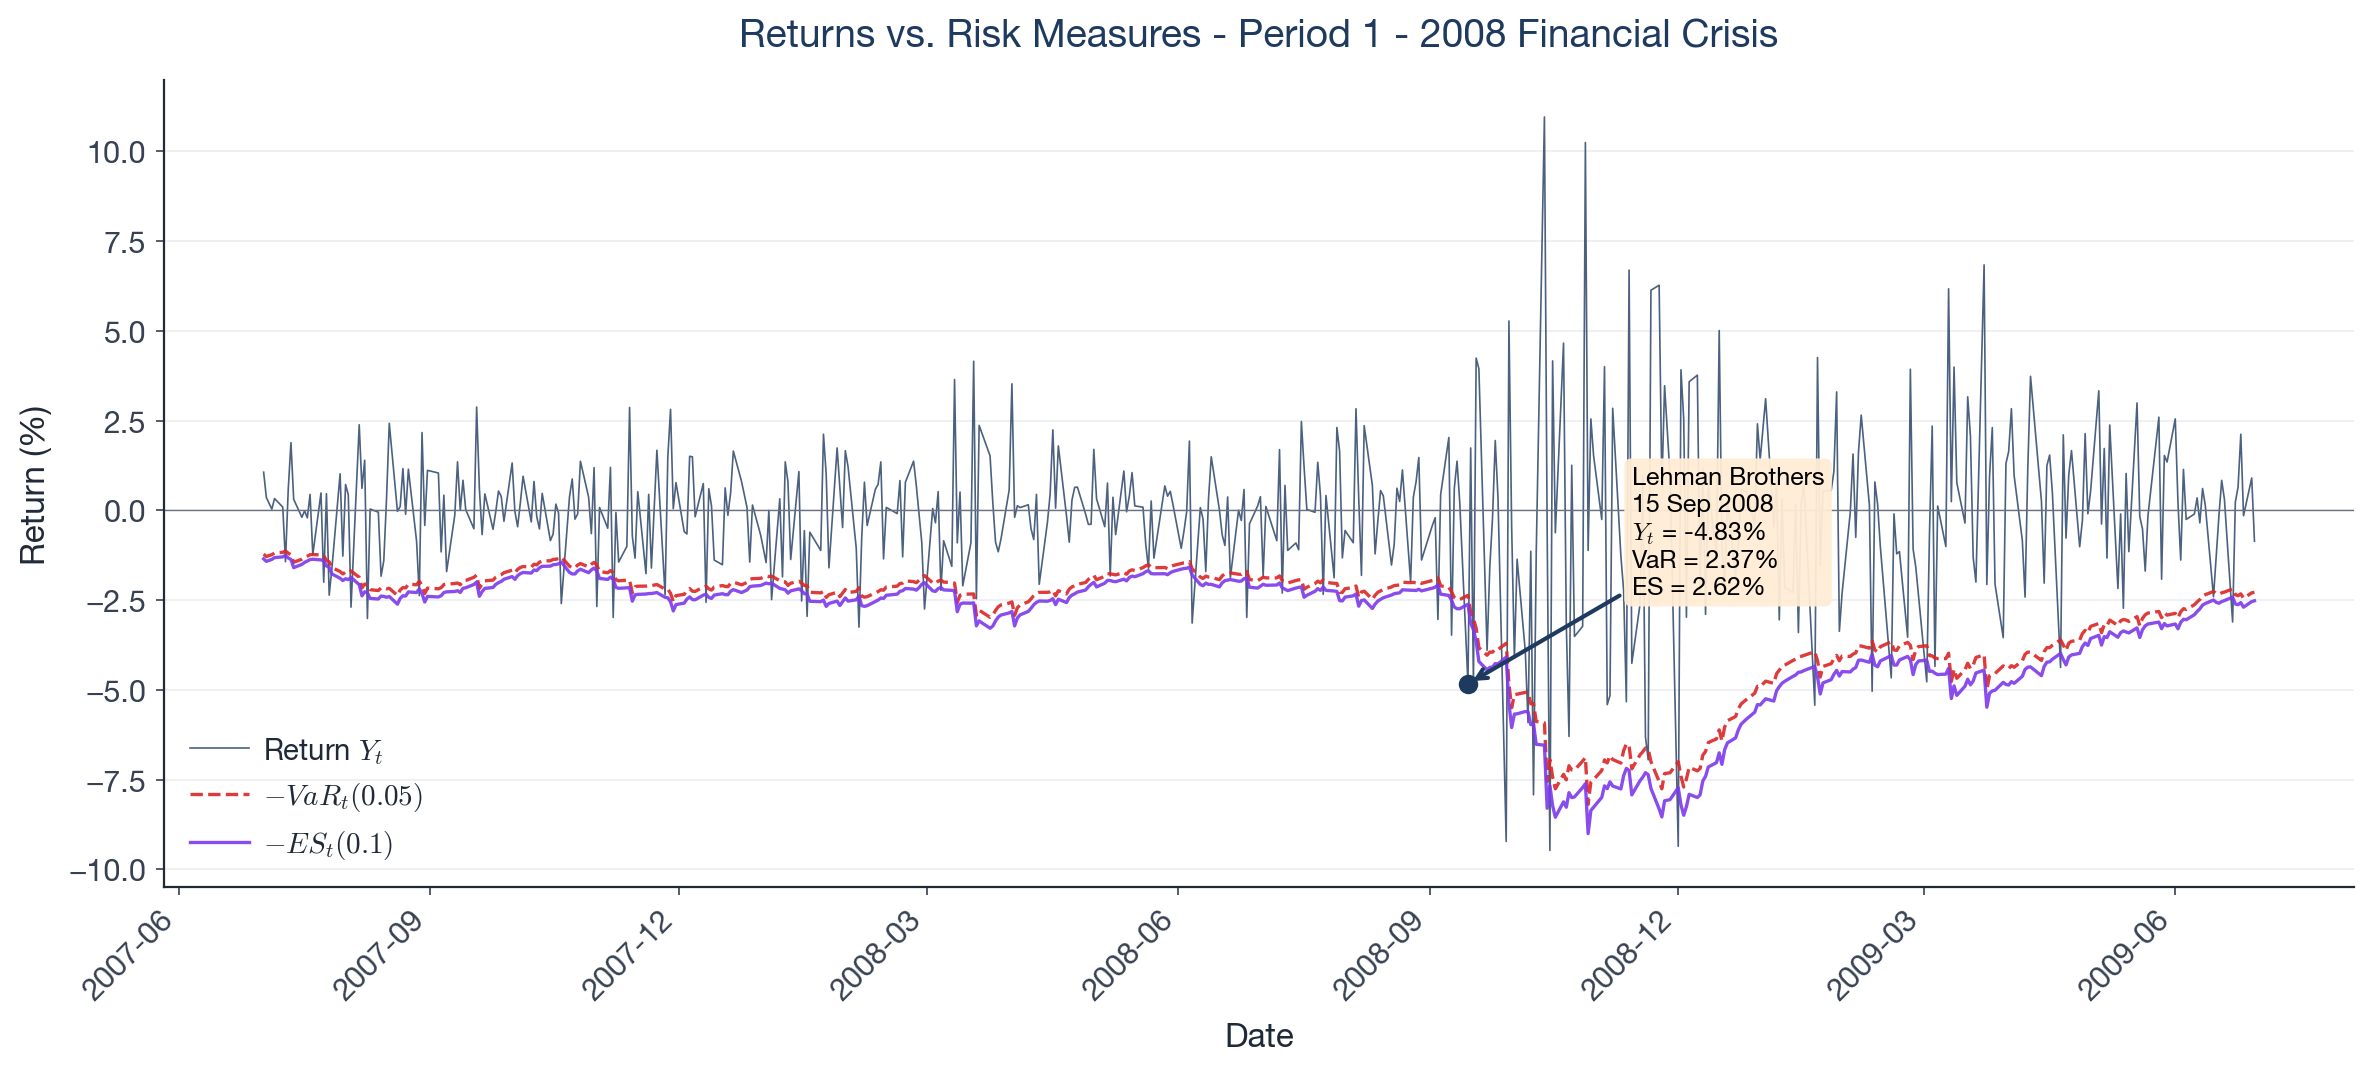
\includegraphics[width=0.95\textwidth]{../assets/figures/01_returns_var_es_2008.png}
\caption{S\&P 500 daily returns and one-step-ahead negative VaR and ES
envelopes over the Global Financial Crisis out-of-sample window
($\alpha_{VaR} = 0.05$, $\alpha_{ES} = 0.10$). The annotation
identifies the 15~September 2008 Lehman Brothers collapse, where the
realised return ($-4.83\%$) exceeded both the VaR ($2.37\%$) and the
ES ($2.62\%$) envelopes.}
\label{fig:returns-var-es}
\end{figure}

\begin{figure}[ht]
\centering
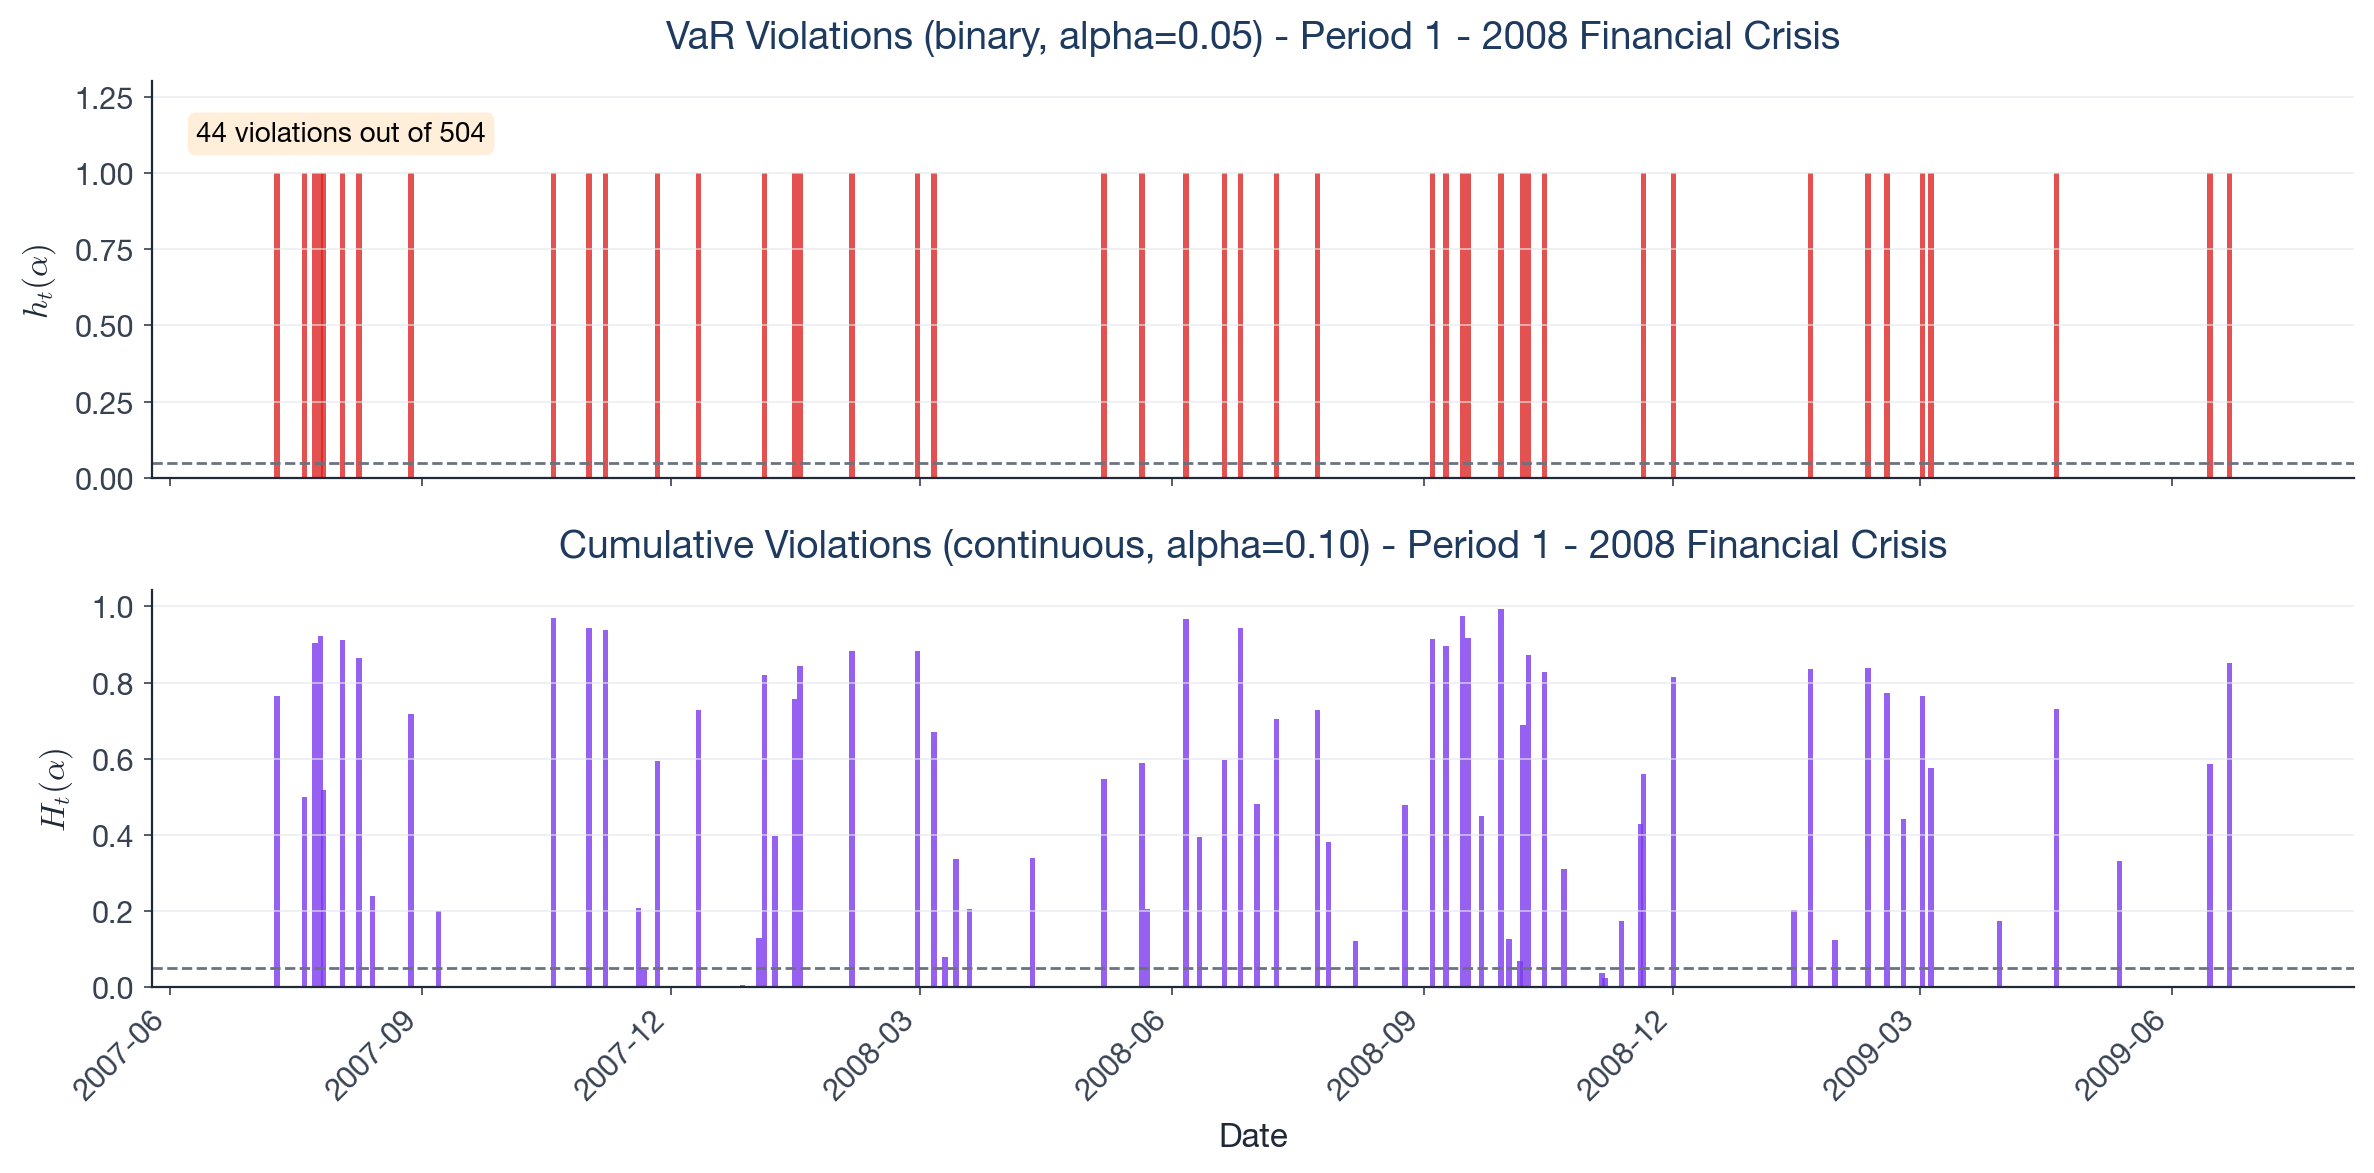
\includegraphics[width=0.95\textwidth]{../assets/figures/01_violations_2008.png}
\caption{Violation indicators over the GFC OOS window. Top: binary
VaR violation indicator $h_t = \one\{u_t \leq \alpha_{VaR}\}$, with the
horizontal line at the nominal rate $\alpha_{VaR} = 0.05$. Bottom:
cumulative ES severity $H_t = \alpha_{ES}^{-1}(\alpha_{ES} - u_t)\,
\one\{u_t \leq \alpha_{ES}\}$, with the horizontal line at the
expectation $\alpha_{ES}/2$ under correct specification.}
\label{fig:violations-2008}
\end{figure}

\begin{figure}[ht]
\centering
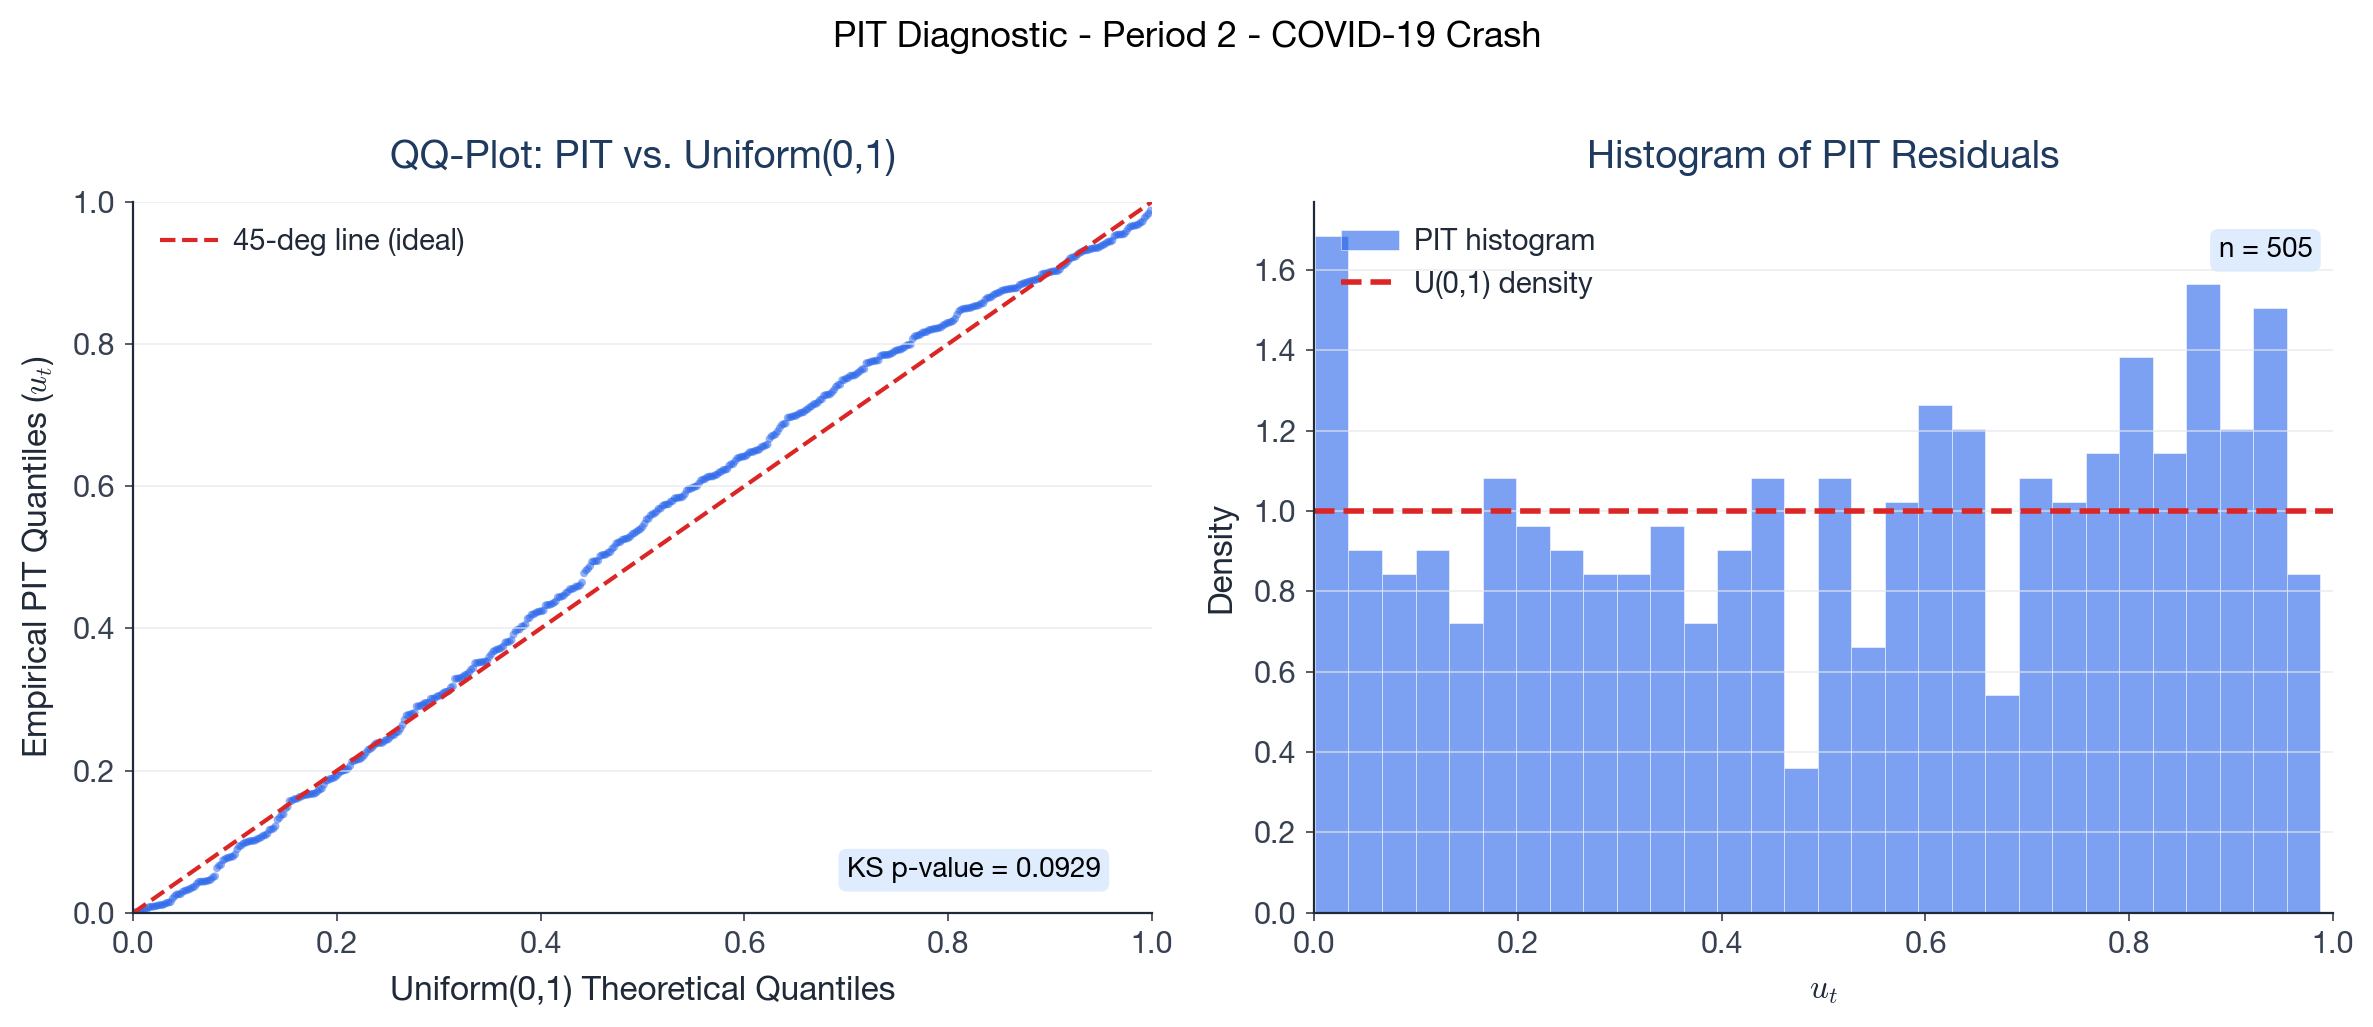
\includegraphics[width=0.95\textwidth]{../assets/figures/01_pit_diagnostic_covid.png}
\caption{PIT residual diagnostic for the COVID-19 OOS window. Left:
QQ-plot of the sorted $u_t$ against uniform quantiles, with the
45-degree reference line. Right: histogram of $u_t$ against the
uniform density. The Kolmogorov--Smirnov test against $\mathrm{Uniform}(0,1)$
returns $p = 0.0929$, so the marginal distribution of $u_t$ is
consistent with correct specification even though six of the eleven
backtests reject the joint hypothesis at $5\%$.}
\label{fig:pit-covid}
\end{figure}

Figure~\ref{fig:returns-var-es} shows the realised returns against
the negative VaR and ES envelopes on the GFC OOS slice;
Figure~\ref{fig:violations-2008} shows the resulting $h_t$ and $H_t$
series. Figure~\ref{fig:pit-covid} reports the PIT residual
diagnostic on the COVID window: the Kolmogorov--Smirnov test against
$\mathrm{Uniform}(0,1)$ returns $p = 0.0929$, so the marginal distribution
of $u_t$ on COVID is consistent with correct specification at $5\%$
even though the joint hypothesis is rejected by ten of the thirteen
tests in Table~\ref{tab:single}. This is precisely the kind of
contrast the battery is designed to expose: marginal-quantile fit can
look acceptable while the conditional dynamics fail at the tail.

\subsection{Multi-asset, multi-crisis grid}
\label{sec:res-grid}

The grid evaluates the basic eleven-test battery on each of the $25$
$(\mathrm{asset},\,\mathrm{crisis})$ cells. The robust variants
$MU_{ES}$ and $MC_{ES}$ are absent from the grid because the
multi-asset harness does not propagate the fitted parameter vector and
the realised in-sample series required for the central-difference
Jacobian. Every cell estimates without numerical issues; the grid
totals $5 \times 5 \times 11 = 275$ p-values.

Table~\ref{tab:grid} reports the rejection rate of each test across
the five assets, period by period. The rejection rate is the share of
assets (out of five) that reject the null at the $5\%$ level on the
given crisis window. The patterns observed on the S\&P 500 in
Section~\ref{sec:res-single} hold across the four pre-2023 windows:
the marginal-coverage block reaches near-unanimous rejection,
$\mathrm{Christoffersen}_{CCI}$ stays at or below $20\%$, and $Z_2$
dominates $Z_1$ by a wide margin.

\begin{table}[ht]
\centering
\caption{Rejection rate per $(\mathrm{test}, \mathrm{crisis})$ cell.
Each entry is the share of assets (out of five) that reject the test
at the $5\%$ level on the given crisis window. The right-most column
totals the four pre-2023 crises (20 cells per test) for compactness.}
\label{tab:grid}
\small
\setlength{\tabcolsep}{6pt}
\begin{tabular}{@{}l*{5}{S[table-format=1.2]}S[table-format=2.0]@{}}
\toprule
\textbf{Test} & {COVID} & {Dotcom} & {GFC} & {Inflation 2022} & {SVB} & {\,\,Pre-SVB rej./20} \\
\midrule
$U_{ES}$              & 1.00 & 1.00 & 1.00 & 1.00 & 0.00 & 20 \\
$C_{ES}(5)$           & 0.40 & 0.40 & 0.60 & 0.40 & 0.00 & 9  \\
$U_{VaR}$             & 0.80 & 1.00 & 1.00 & 1.00 & 0.00 & 19 \\
$C_{VaR}(5)$          & 0.20 & 0.40 & 0.40 & 0.40 & 0.00 & 7  \\
$Z_1$                 & 0.40 & 0.00 & 0.60 & 0.00 & 0.00 & 5  \\
$Z_2$                 & 1.00 & 0.80 & 1.00 & 1.00 & 0.20 & 19 \\
$\mathrm{McNeil}\text{--}\mathrm{Frey}$ & 0.40 & 0.20 & 0.60 & 0.20 & 0.20 & 7 \\
$\mathrm{Kupiec}_{POF}$       & 0.80 & 1.00 & 1.00 & 1.00 & 0.00 & 19 \\
$\mathrm{Christoffersen}_{CCI}$ & 0.00 & 0.00 & 0.20 & 0.20 & 0.00 & 2 \\
$\mathrm{Christoffersen}_{CC}$  & 0.60 & 1.00 & 1.00 & 1.00 & 0.00 & 18 \\
$\mathrm{KLM}_{\text{mult}}(4)$ & 1.00 & 1.00 & 1.00 & 1.00 & 0.00 & 20 \\
\bottomrule
\end{tabular}
\end{table}

\begin{figure}[ht]
\centering
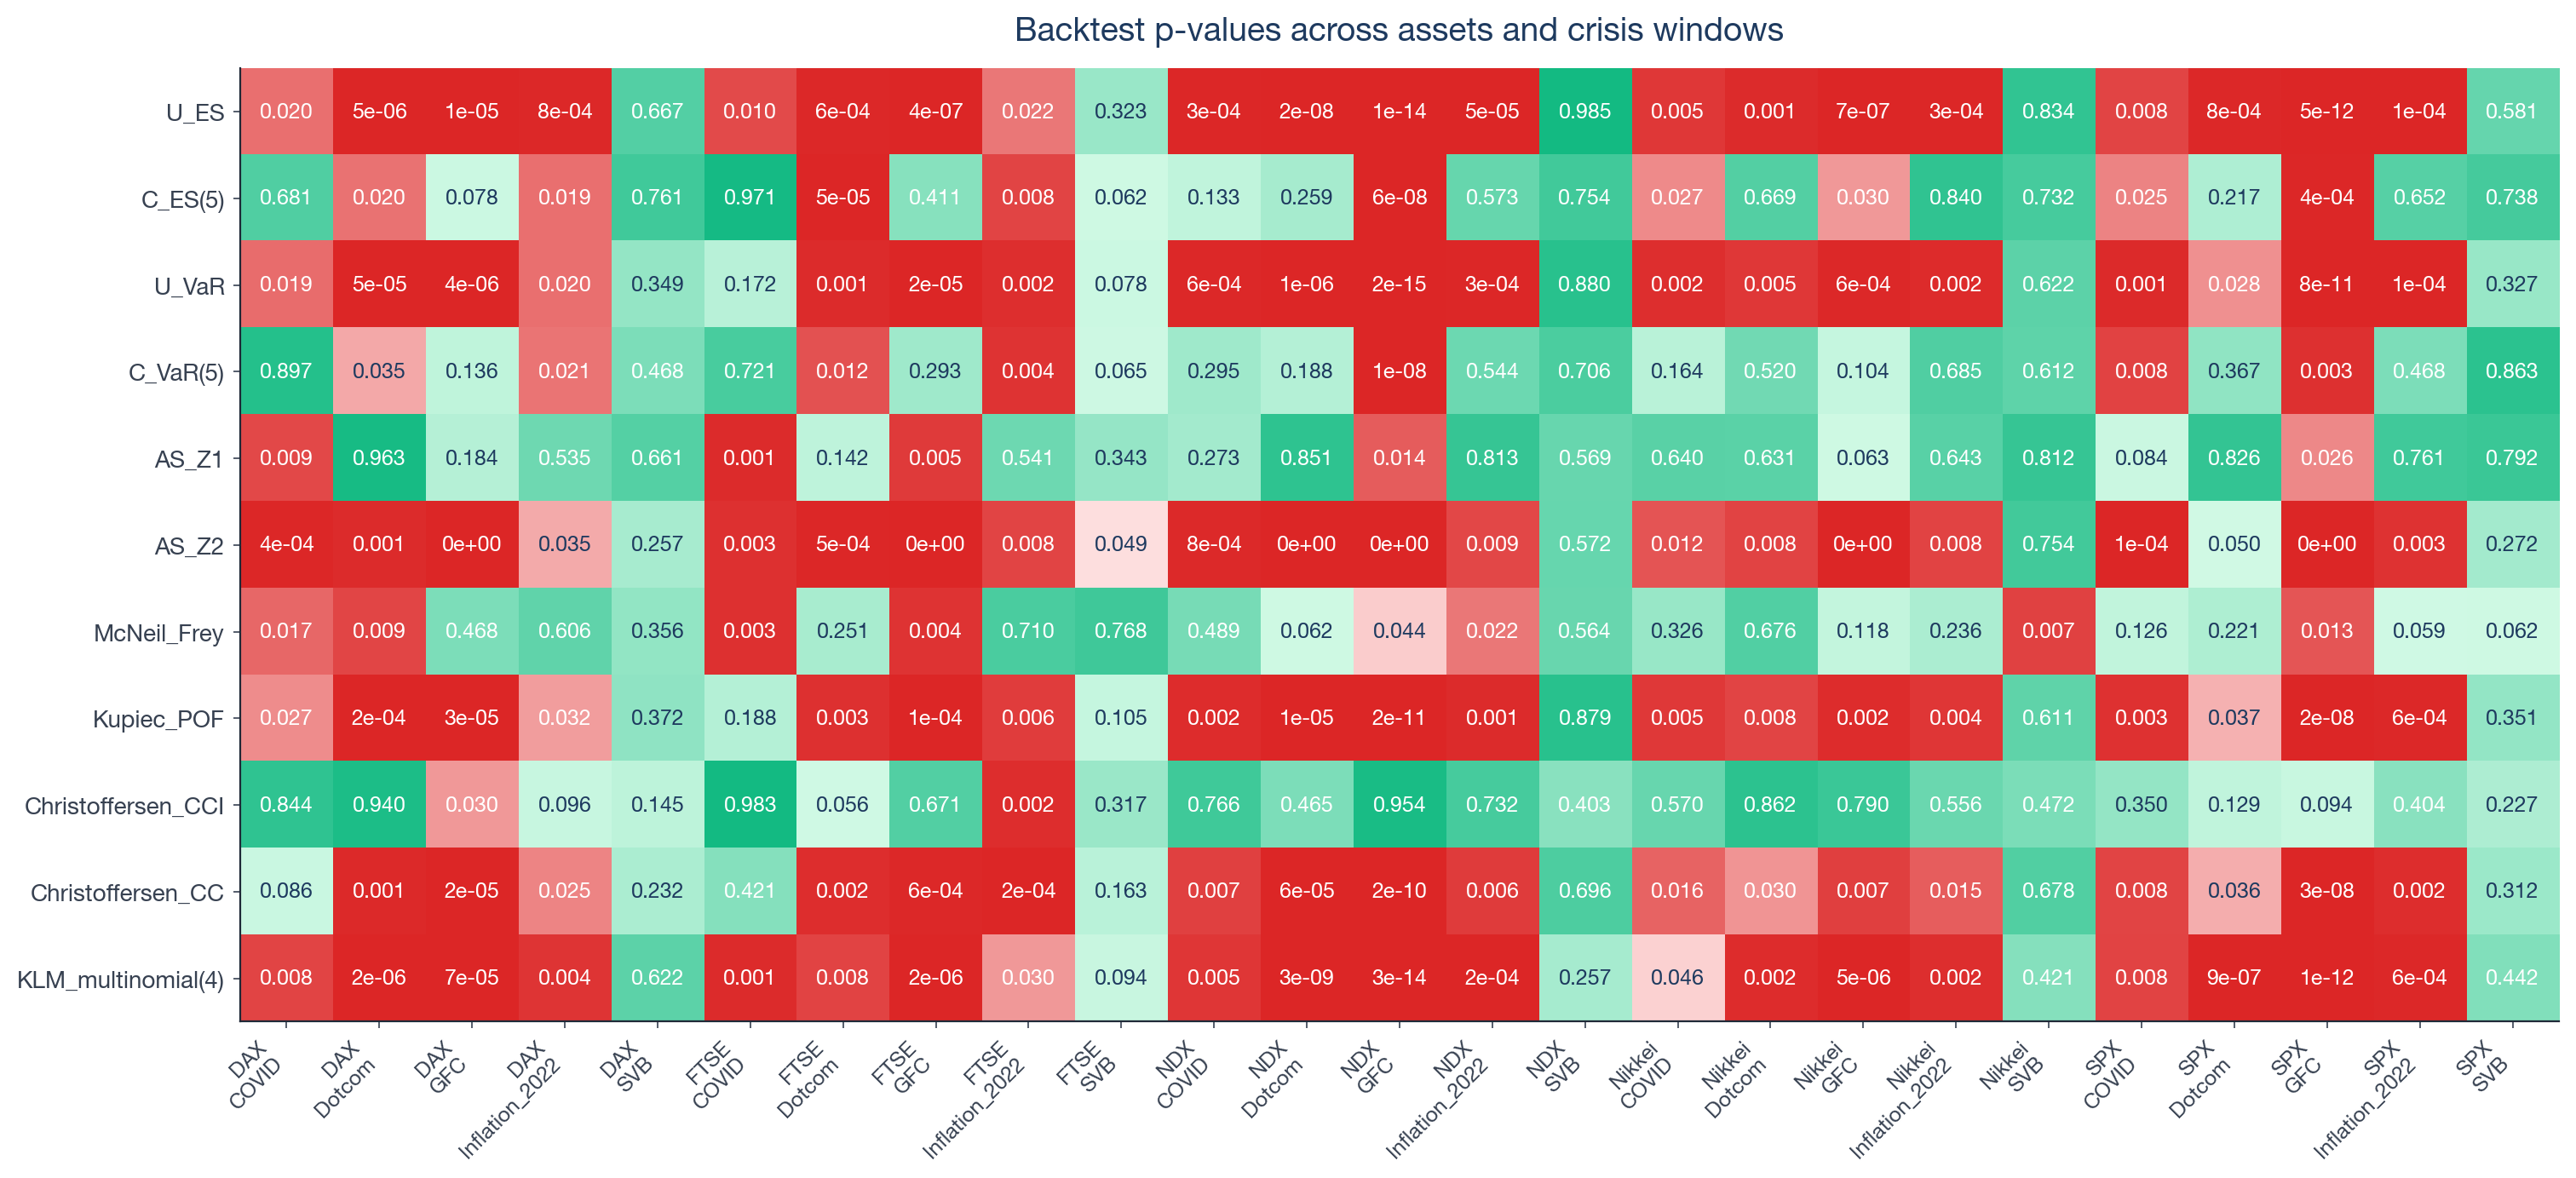
\includegraphics[width=0.98\textwidth]{../assets/figures/02_battery_heatmap.png}
\caption{Heatmap of p-values across $(\mathrm{test}) \times
(\mathrm{asset},\,\mathrm{crisis})$ cells. Cells with $p < 0.05$ are
shaded red, cells failing to reject are shaded green; the intensity
tracks distance from the threshold. Eleven tests $\times$ twenty-five
cells gives $275$ p-values.}
\label{fig:heatmap}
\end{figure}

\begin{figure}[ht]
\centering
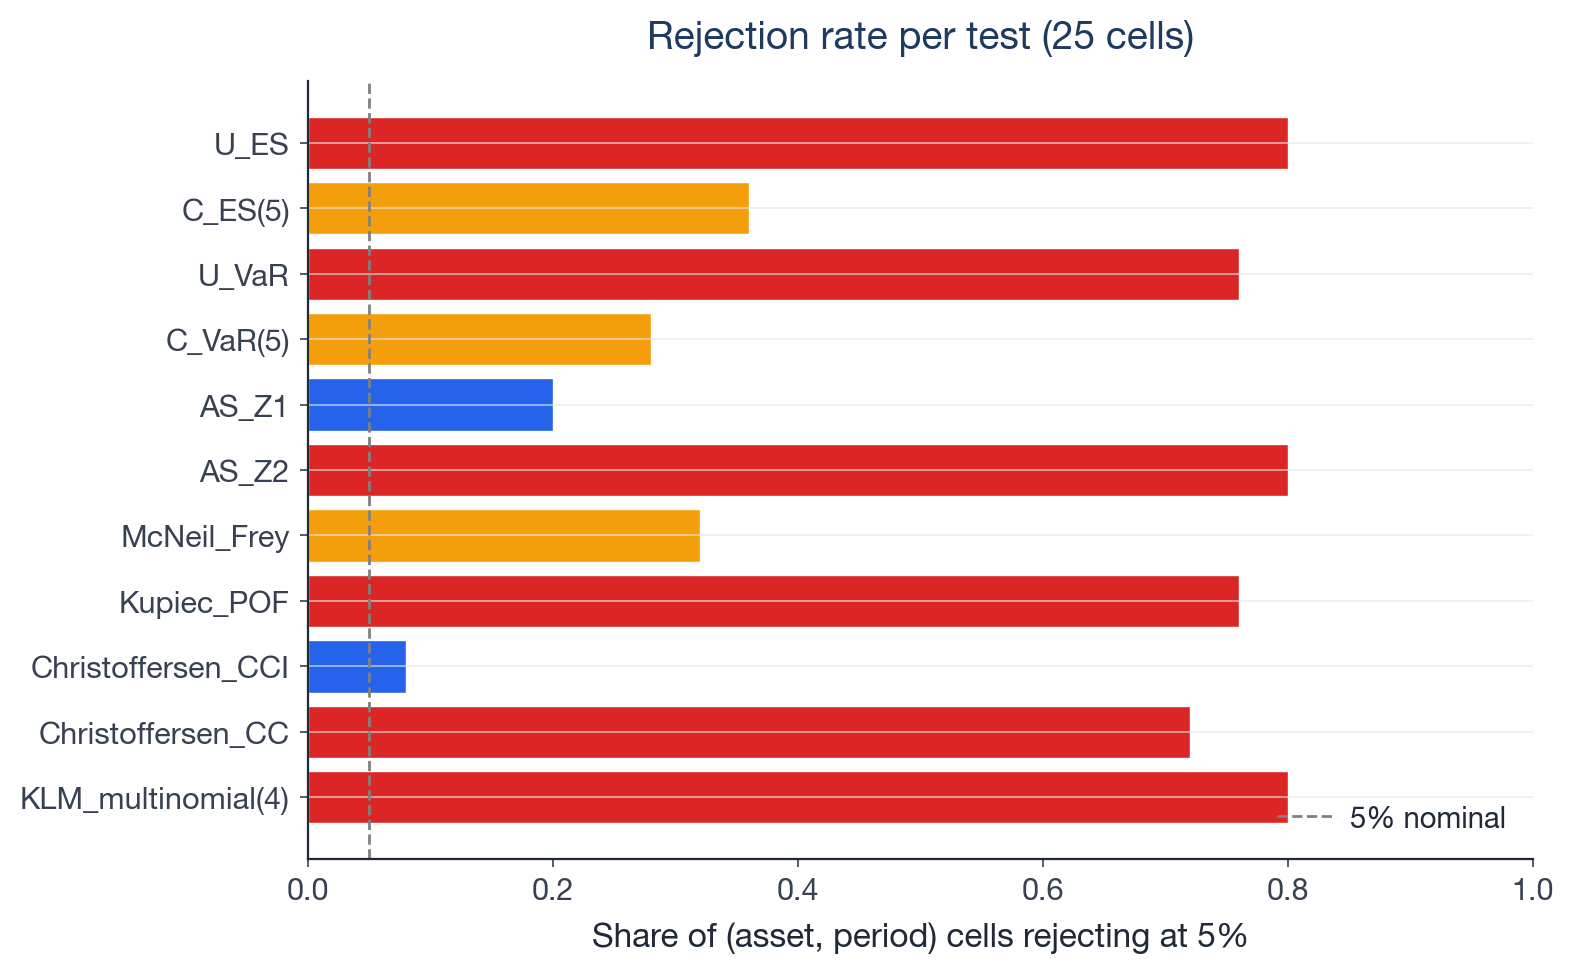
\includegraphics[width=0.85\textwidth]{../assets/figures/02_reject_rate_per_test.png}
\caption{Share of the $25$ $(\mathrm{asset},\,\mathrm{crisis})$ cells
in which each test rejects at the $5\%$ level. The vertical line at
$5\%$ marks the size a correctly-specified test should achieve under
the null.}
\label{fig:reject-per-test}
\end{figure}

Two patterns stand out. First, the SVB column is quiet: of the $55$ test--asset cells on the SVB window, only $2$
reject (one $Z_2$, one McNeil--Frey). The 2023 banking shock saw
sharp moves in regional bank equities but limited index-level
volatility, so the AR(1)-GARCH(1,1)-$t$ scales its envelope correctly.
This is a useful sanity check: a window labelled ``crisis'' does not
have to coincide with ES mis-specification on diversified indices.

Second, the gap between $\mathrm{Christoffersen}_{CCI}$ ($2/20$
rejections outside SVB) and $\mathrm{Christoffersen}_{CC}$ ($18/20$)
is carried almost entirely by $\mathrm{LR}_{POF}$, which on its own
rejects $19/20$ cells. The decomposition $\mathrm{LR}_{CC} =
\mathrm{LR}_{POF} + \mathrm{LR}_{IND}$ is exact, and the empirical
evidence assigns the rejection signal to the marginal-coverage
component. The day-to-day independence component contributes a single
extra rejection on the GFC and on the inflation window. Pooling the
two components into $\mathrm{LR}_{CC}$ thus inflates the apparent
power of the joint test, but the source of the rejection is the
violation count, not the clustering pattern.

Figure~\ref{fig:heatmap} renders the full $11 \times 25$ p-value
grid; Figure~\ref{fig:reject-per-test} aggregates over the $25$ cells
to give a per-test summary.

\subsection{Monte Carlo size-and-power study}
\label{sec:res-mc}

The Monte Carlo study evaluates the finite-sample behaviour of each
test under four scenarios:
\begin{itemize}
  \item $H_0^{(t)}$: AR(1)-GARCH(1,1)-$t$ with $\nu = 8.0$
    (correctly specified).
  \item $H_1^{(\gamma=0.15)}$: GJR-GARCH(1,1,1)-$t$ with $\gamma = 0.15$
    (moderate asymmetric leverage).
  \item $H_1^{(\gamma=0.25)}$: GJR-GARCH(1,1,1)-$t$ with $\gamma = 0.25$
    (strong asymmetric leverage).
  \item $H_1^{(\mathcal{N})}$: AR(1)-GARCH(1,1)-$\mathcal{N}$
    (Gaussian innovations, same volatility dynamics).
\end{itemize}
For each scenario and each sample size $n \in \{250, 500, 1{,}000,
2{,}500\}$ the study draws $1{,}000$ replications, fits an
AR(1)-GARCH(1,1)-$t$ on the first $60\%$ of each path, and runs the
basic eleven-test battery on the remaining $40\%$. The $Z_1$ and $Z_2$
p-values are parametric Monte-Carlo readings from a
\code{StandardizedTSimulator} with $2{,}000$ draws per replication;
the McNeil--Frey bootstrap uses $200$ block-bootstrap samples per
replication in the Monte-Carlo study (vs.~$10{,}000$ in the CLI runs)
to keep the grid affordable. The full size-and-power log contains
$176{,}000$ rows; the snapshot at $n = 1{,}000$ is reported in
Table~\ref{tab:mc}.

\begin{table}[ht]
\centering
\caption{Empirical rejection rate at $n = 1{,}000$. Columns: rejection
rate under the correctly-specified DGP ($H_0$) and under the three
alternatives. Values in bold sit at or above $25\%$; values in
italics deviate from the nominal $5\%$ by more than $4$~pp under
$H_0$ (size distortion).}
\label{tab:mc}
\small
\setlength{\tabcolsep}{8pt}
\begin{tabular}{@{}l*{4}{S[table-format=1.2]}@{}}
\toprule
\textbf{Test} & {$H_0$: GARCH-$t$} & {$H_1$: GJR $\gamma{=}.15$} & {$H_1$: GJR $\gamma{=}.25$} & {$H_1$: Normal} \\
\midrule
$U_{ES}$              & {\itshape 0.16} & 0.17 & \textbf{0.31} & 0.17 \\
$C_{ES}(5)$           & 0.08 & 0.16 & \textbf{0.30} & 0.09 \\
$U_{VaR}$             & {\itshape 0.14} & 0.13 & \textbf{0.28} & 0.15 \\
$C_{VaR}(5)$          & 0.08 & 0.14 & 0.24 & 0.07 \\
$Z_1$                 & {\itshape 0.12} & 0.10 & 0.12 & 0.07 \\
$Z_2$                 & {\itshape 0.14} & 0.14 & 0.23 & 0.12 \\
$\mathrm{McNeil}\text{--}\mathrm{Frey}$ & {\itshape 0.16} & 0.16 & 0.14 & 0.14 \\
$\mathrm{Kupiec}_{POF}$         & {\itshape 0.13} & 0.14 & \textbf{0.26} & 0.15 \\
$\mathrm{Christoffersen}_{CCI}$ & 0.04 & 0.05 & 0.10 & 0.04 \\
$\mathrm{Christoffersen}_{CC}$  & {\itshape 0.12} & 0.13 & \textbf{0.26} & 0.11 \\
$\mathrm{KLM}_{\text{mult}}(4)$ & {\itshape 0.13} & 0.15 & \textbf{0.25} & 0.13 \\
\bottomrule
\end{tabular}
\end{table}

\begin{figure}[ht]
\centering
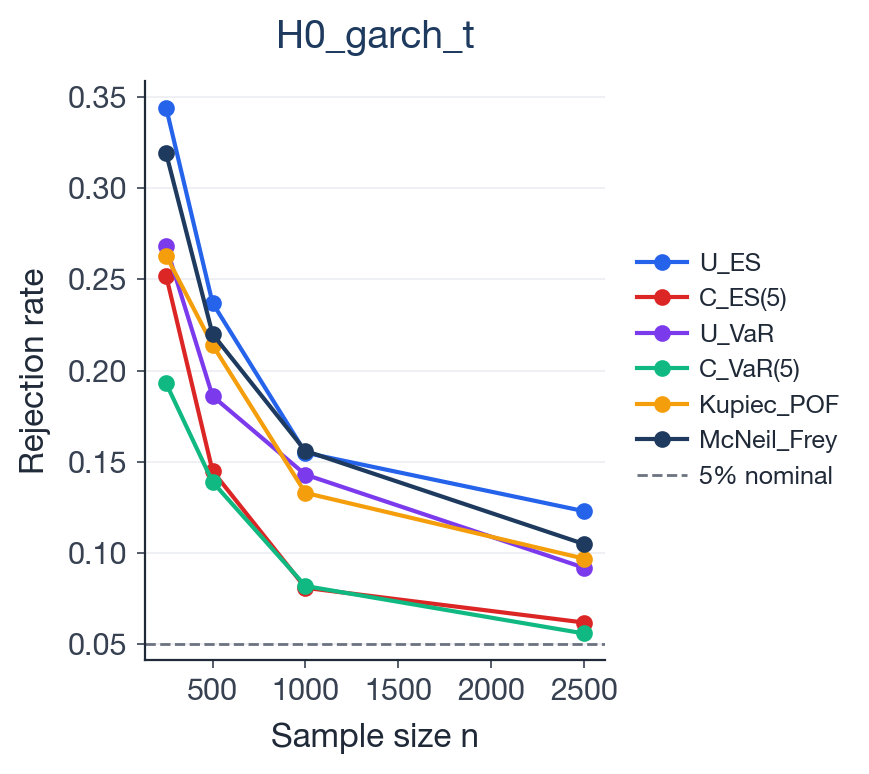
\includegraphics[width=0.7\textwidth]{../assets/figures/03_size_under_h0.png}
\caption{Empirical size of six representative tests under the
correctly-specified DGP, as a function of the OOS sample size $n$.
The dashed line marks the nominal $5\%$ level.}
\label{fig:size}
\end{figure}

\begin{figure}[ht]
\centering
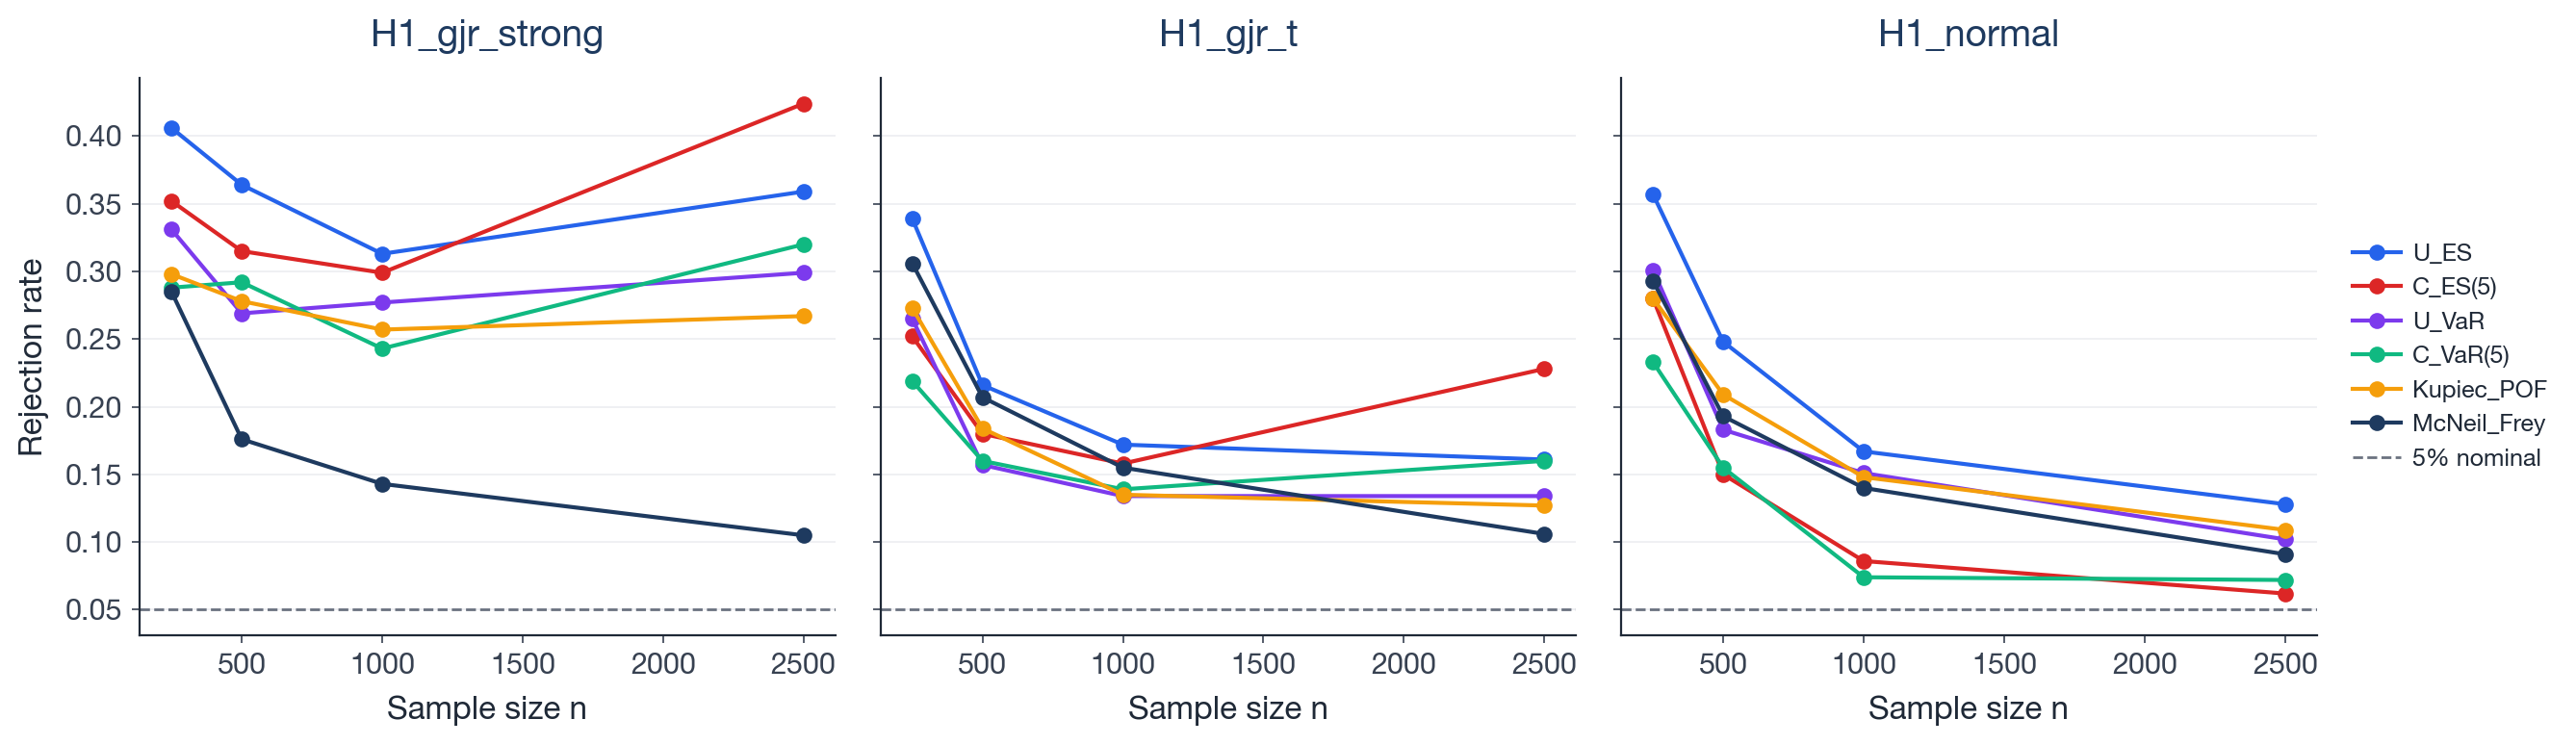
\includegraphics[width=0.98\textwidth]{../assets/figures/03_power_curves.png}
\caption{Empirical power curves of six representative tests under the
three alternative DGPs (left to right: strong GJR leverage, moderate
GJR leverage, Gaussian innovations), as a function of the OOS sample
size $n$. The dashed line marks the nominal $5\%$ level.}
\label{fig:power}
\end{figure}

Under the correctly-specified DGP the conditional Box--Pierce tests
$C_{ES}(5)$ and $C_{VaR}(5)$ ($0.08$) and the day-to-day independence
test $\mathrm{Christoffersen}_{CCI}$ ($0.04$) are within four
percentage points of the nominal $5\%$ size. The remaining eight
tests over-reject: $U_{ES}$ and McNeil--Frey at $0.16$, $U_{VaR}$ and
$Z_2$ at $0.14$, $\mathrm{Kupiec}_{POF}$ and
$\mathrm{KLM}_{\text{mult}}(4)$ at $0.13$, $Z_1$ and
$\mathrm{Christoffersen}_{CC}$ at $0.12$. The over-rejection narrows
but does not vanish at $n = 2{,}500$ (Figure~\ref{fig:size}),
consistent with the slow convergence of the asymptotic $\chi^2$
approximations for marginal-coverage tests.

Under the moderate leverage alternative ($\gamma = 0.15$) all
rejection rates stay below $20\%$. Under the strong leverage
alternative ($\gamma = 0.25$) the conditional Box-Pierce block leads:
$U_{ES}$ at $0.31$, $C_{ES}(5)$ at $0.30$, $U_{VaR}$ at $0.28$,
$\mathrm{Kupiec}_{POF}$ and $\mathrm{Christoffersen}_{CC}$ at
$0.26$, $\mathrm{KLM}_{\text{mult}}(4)$ at $0.25$, $C_{VaR}(5)$ at
$0.24$, $Z_2$ at $0.23$. The net power (rejection rate at $H_1$
minus rejection rate at $H_0$) is +$22$~pp for $C_{ES}(5)$, +$16$~pp
for $C_{VaR}(5)$, +$15$~pp for $U_{ES}$, +$14$~pp for $U_{VaR}$ and
$\mathrm{Christoffersen}_{CC}$, +$13$~pp for $\mathrm{Kupiec}_{POF}$,
+$12$~pp for $\mathrm{KLM}_{\text{mult}}(4)$, +$9$~pp for $Z_2$,
+$6$~pp for $\mathrm{Christoffersen}_{CCI}$, $0$~pp for $Z_1$, and
$-2$~pp for McNeil--Frey. The conditional Box-Pierce statistics on
cumulative violations are the most powerful of the eleven tests
against leverage misspecification.

The $Z_1$ versus $Z_2$ contrast is sharp: at $n = 1{,}000$, $Z_2$ has
net power $+9$~pp under strong leverage while $Z_1$ has $0$~pp. The
gap reflects that $Z_2$ aggregates the loss-to-ES ratio over the full
OOS window and so picks up an excess number of violations, while
$Z_1$ normalises only over the empirical violation set and remains
blind to that channel. Practitioners reaching for ``the
Acerbi--Szekely test'' should be aware that the two variants behave
very differently against asymmetric leverage.

Under the Gaussian-innovation alternative every rejection rate stays
within $4$~pp of its $H_0$ value, including the three tests
specifically designed to track tail mis-specification ($Z_1$, $Z_2$,
McNeil--Frey). At $n = 1{,}000$ the mismatch between a Gaussian tail
and a Student-$t$ tail predicted by the fitted model is not pronounced
enough in the PIT residuals to register on any of the $u_t$-based
tests; sharper detection requires a larger $n$ or a heavier-tailed
alternative. Power curves over $n \in \{250, 500, 1{,}000, 2{,}500\}$
are shown in Figure~\ref{fig:power}.

\subsection{LSTM-Quantile versus AR(1)-GARCH(1,1)-$t$ on COVID-19}
\label{sec:res-lstm}

The neural baseline compares an LSTM-Quantile head to the
AR(1)-GARCH(1,1)-$t$ baseline on the COVID-19 OOS slice. Both models
are evaluated at $\alpha = 0.05$. The LSTM is trained on
the 2010-2019 S\&P 500 in-sample window ($n_{\text{IS}} = 2{,}516$
days) for $30$ epochs with sequence length $L = 20$, hidden size
$32$, batch size $64$, Adam at learning rate $10^{-3}$, and a joint
pinball $+$ FZ0 loss. The training runs on Apple's MPS accelerator;
the final pinball loss is $0.7906$ and the final FZ0 loss is
$0.8943$. Both models emit one-step-ahead $(\VaR_t, \ES_t)$ for every
OOS day ($n_{\text{OOS}} = 505$).

\begin{table}[ht]
\centering
\caption{Mean VaR and ES forecasts over the COVID-19 OOS slice. The
LSTM trained on 2010--2019 under-calls VaR by a factor of
$2.63$.}
\label{tab:lstm-mean}
\small
\begin{tabular}{@{}lcc@{}}
\toprule
\textbf{Model} & \textbf{Mean VaR (\%)} & \textbf{Mean ES (\%)} \\
\midrule
AR(1)-GARCH(1,1)-$t$ & 1.831 & 2.682 \\
LSTM-Quantile        & 0.695 & 2.839 \\
\bottomrule
\end{tabular}
\end{table}

\begin{table}[ht]
\centering
\caption{Battery comparison on the COVID-19 OOS slice. Five tests
that do not require an analytical PIT are reported; the
Acerbi--Szekely p-values would need a parametric simulator of the
LSTM forecast distribution, which is not available.}
\label{tab:lstm-battery}
\small
\setlength{\tabcolsep}{8pt}
\begin{tabular}{@{}l S[table-format=3.3] S[table-format=1.4] c S[table-format=-3.3] S[table-format=1.4] c@{}}
\toprule
& \multicolumn{3}{c}{\textbf{GARCH-$t$}} & \multicolumn{3}{c}{\textbf{LSTM}} \\
\cmidrule(lr){2-4}\cmidrule(lr){5-7}
\textbf{Test} & {Stat.} & {p-value} & Decision & {Stat.} & {p-value} & Decision \\
\midrule
$\mathrm{Kupiec}_{POF}$         & 7.762   & 0.0053 & \textbf{R} & 150.636 & 0.0000 & \textbf{R} \\
$\mathrm{Christoffersen}_{CCI}$ & 1.084   & 0.2979 & F          & 0.468   & 0.4941 & F          \\
$\mathrm{Christoffersen}_{CC}$  & 8.846   & 0.0120 & \textbf{R} & 151.103 & 0.0000 & \textbf{R} \\
$Z_1$                           & 0.099   & {N/A}  & ---        & -0.348  & {N/A}  & ---        \\
$Z_2$                           & 0.741   & {N/A}  & ---        & 1.685   & {N/A}  & ---        \\
\bottomrule
\end{tabular}
\end{table}

\begin{figure}[ht]
\centering
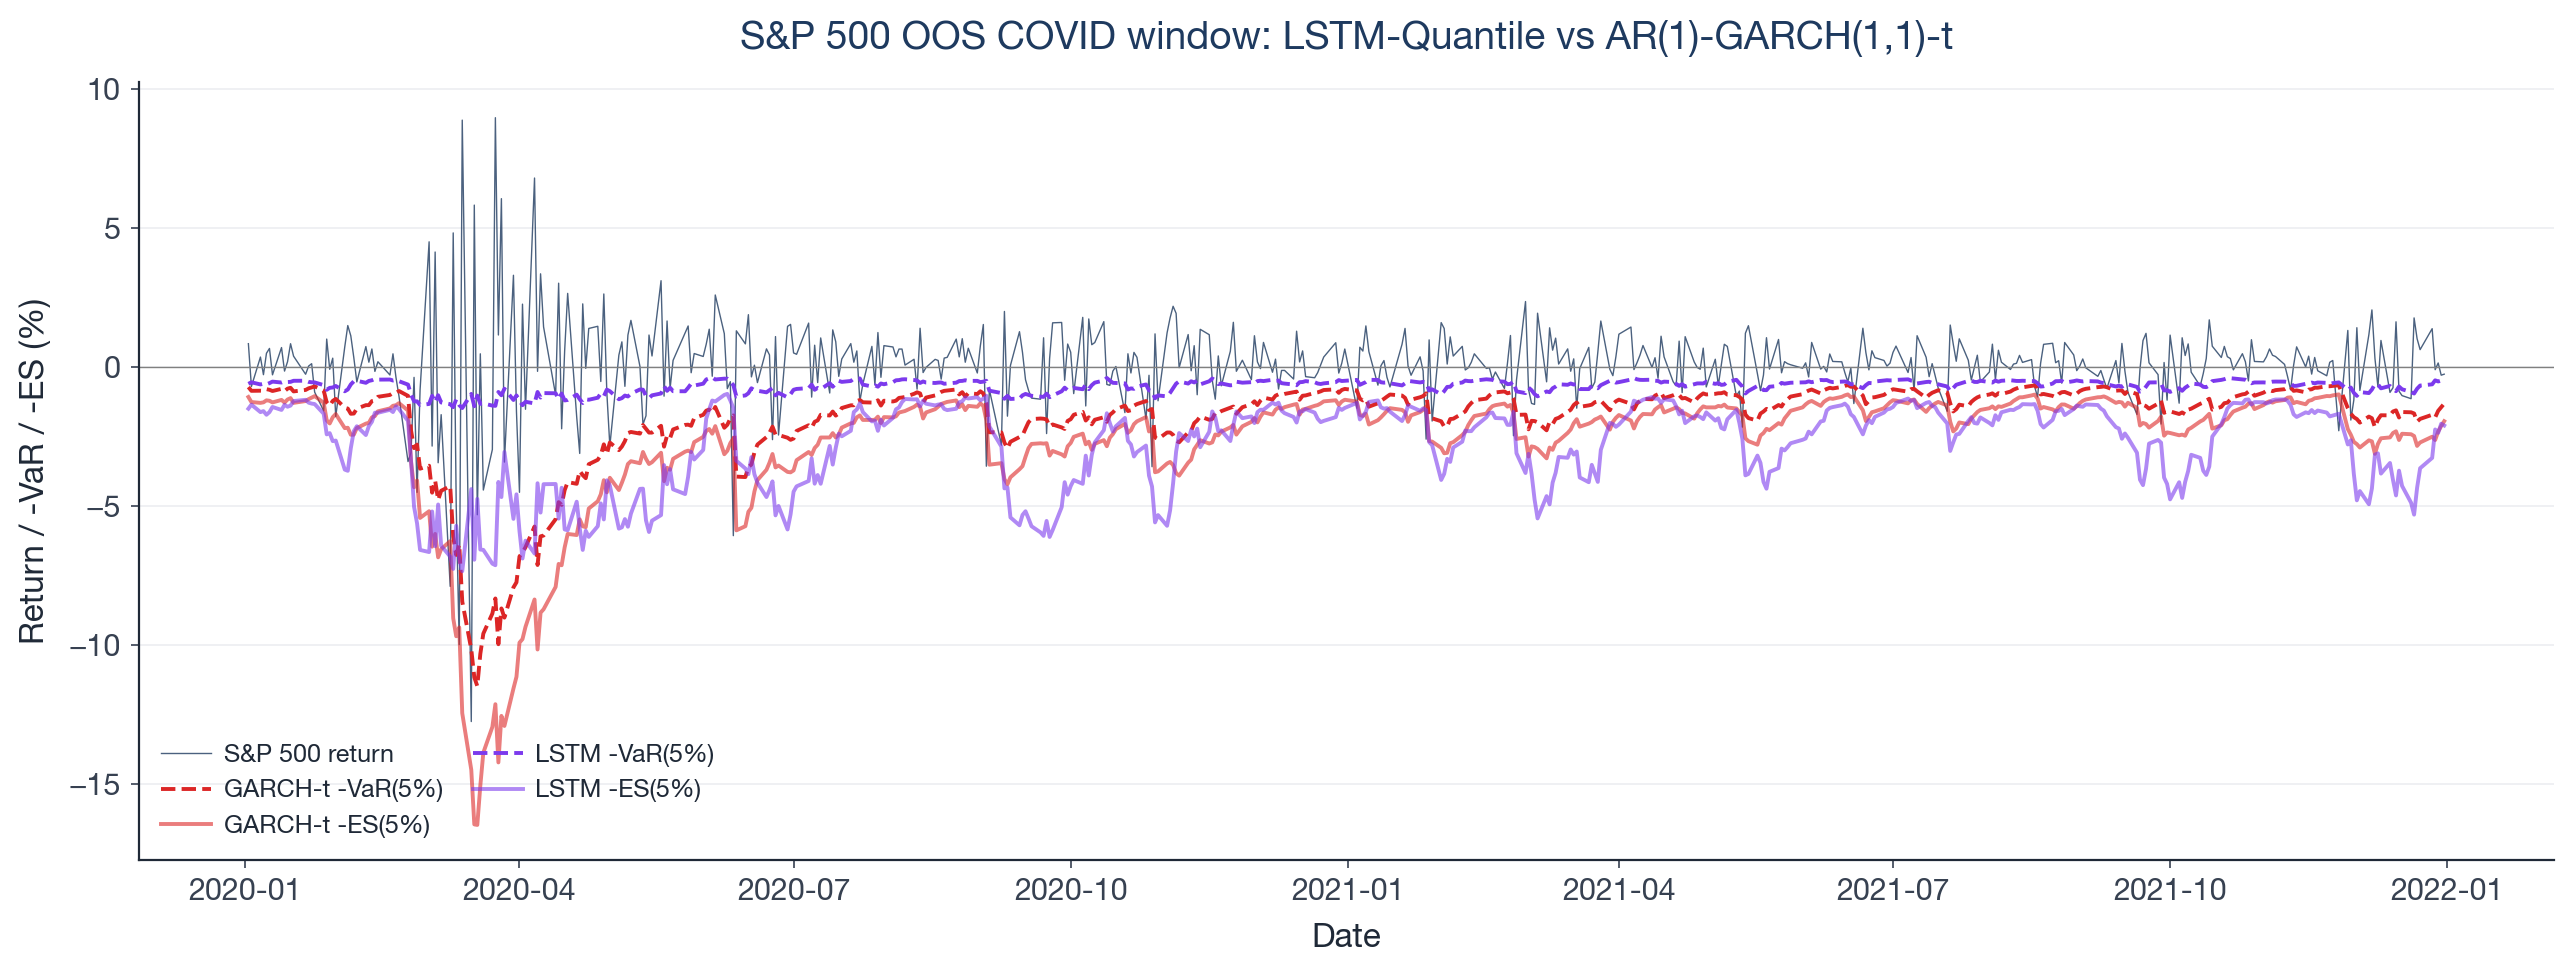
\includegraphics[width=0.98\textwidth]{../assets/figures/04_lstm_vs_garch_covid.png}
\caption{S\&P 500 daily returns over the COVID-19 OOS slice
($2020$--$2021$) with the negative VaR and ES envelopes of the
AR(1)-GARCH(1,1)-$t$ baseline and of the LSTM-Quantile head. The
LSTM, trained on the calm 2010--2019 decade, holds its envelope close
to that decade's level and is consistently breached during the
March~2020 spike.}
\label{fig:lstm-garch}
\end{figure}

Table~\ref{tab:lstm-mean} reports the mean VaR and ES forecasts over
the OOS slice. The LSTM under-calls VaR by a factor of $1.831 / 0.695
= 2.63$: trained on the calm 2010--2019 decade, it produces a VaR
envelope anchored to that regime's volatility level rather than to
the realised regime during the OOS slice. The mean ES values are
closer ($2.682$ vs.~$2.839$), but the LSTM's VaR-to-ES spread is much
wider than the GARCH's, an artefact of the softplus parameterisation
that decouples the two heads on tail days.

Table~\ref{tab:lstm-battery} reports the subset of the battery that
does not require an analytical PIT. Both models reject the Kupiec POF
test, but the LSTM's statistic is $150.636$ versus the GARCH's
$7.762$, a factor of $19.4$. The Christoffersen independence
component fails to reject for either model, so the violation rate is
elevated on both but the violations are not consecutively clustered
in the sense of the two-state Markov chain. The Acerbi--Szekely
statistics are reported but their p-values would require a parametric
simulator of the LSTM's forecast distribution, which the
softplus-quantile head does not provide; a mixture-density variant
would supply the missing PIT and is left as future work.

The visual contrast in Figure~\ref{fig:lstm-garch} makes the point:
the GARCH envelope tracks the regime shift in March~2020 by
construction, while the LSTM envelope holds approximately constant.
The neural baseline does not generalise to a once-in-a-decade tail
event when trained on a regime that does not contain one.

\subsection{Mixture-density LSTM: closed-form CDF and the full battery}
\label{sec:res-mdn}

The LSTM-Quantile head produces $(\widehat{\VaR}, \widehat{\ES})$ and
nothing else. Six of the thirteen statistics in
Table~\ref{tab:single} require the PIT residual $u_t = F_t(Y_t)$ or a
parametric simulator, which a quantile-only head cannot supply. The
mixture-density LSTM (MDN-LSTM) replaces the two-output head with
three linear heads on the same LSTM backbone, parameterising the
Student-$t$ distribution of the next return $Y_{t+1} \sim
t_{\nu_t}(\mu_t, \sigma_t)$. The training loss is the negative
log-likelihood of the predicted distribution. From the trained
network, the PIT, the analytic VaR and the analytic ES follow in
closed form; a per-day simulator generates fresh Student-$t$ paths
for the Acerbi--Szekely Monte-Carlo p-values. The robust
Du--Escanciano statistics ($MU_{ES}$, $MC_{ES}$) remain unreachable
because they require the parameter covariance of an MLE fit, which
the stochastic-gradient-trained network does not expose in closed
form.

Trained on the same 2010-2019 window as the LSTM-Quantile and
GARCH-$t$ baselines, the MDN-LSTM converges to a final NLL of
$1.121$ and produces an OOS mean VaR of $1.445\%$ over the COVID-19
window. That sits between the LSTM-Quantile's $0.695\%$ and the
GARCH-$t$'s $1.831\%$ (Table~\ref{tab:mdn-mean}): the MDN scales the
envelope substantially better than the LSTM-Quantile but still
under-calls relative to GARCH-$t$. Average conditional parameters on
the OOS slice are $\bar\mu = 0.11$, $\bar\sigma = 0.77$, $\bar\nu =
4.67$ -- a fat-tailed regime, consistent with what the
GARCH-$t$ fit reports on the same window ($\hat\nu = 4.83$).

\begin{table}[ht]
\centering
\caption{Mean VaR and ES forecasts on the COVID-19 OOS slice,
$\alpha = 0.05$. The MDN-LSTM sits between the LSTM-Quantile and the
GARCH-$t$ baseline; the LSTM-Quantile under-calls VaR by a factor of
$2.63$ relative to GARCH-$t$, the MDN by a factor of $1.27$.}
\label{tab:mdn-mean}
\small
\begin{tabular}{@{}lcc@{}}
\toprule
\textbf{Model} & \textbf{Mean VaR (\%)} & \textbf{Mean ES (\%)} \\
\midrule
AR(1)-GARCH(1,1)-$t$ & 1.831 & 2.682 \\
LSTM-Quantile        & 0.695 & 2.839 \\
MDN-LSTM             & 1.445 & 2.136 \\
\bottomrule
\end{tabular}
\end{table}

\begin{table}[ht]
\centering
\caption{Battery comparison on COVID-19 OOS, $\alpha = 0.05$. The
GARCH-$t$ column reports thirteen statistics (including the two
robust Du--Escanciano variants); the MDN-LSTM column reports
eleven (the robust pair is unavailable). \textbf{R}: reject at
$5\%$. F: fail to reject.}
\label{tab:mdn-battery}
\small
\setlength{\tabcolsep}{6pt}
\begin{tabular}{@{}l S[table-format=2.3] S[table-format=1.4] c S[table-format=2.3] S[table-format=1.4] c@{}}
\toprule
& \multicolumn{3}{c}{\textbf{GARCH-$t$}} & \multicolumn{3}{c}{\textbf{MDN-LSTM}} \\
\cmidrule(lr){2-4}\cmidrule(lr){5-7}
\textbf{Test} & {Stat.} & {p-value} & Dec. & {Stat.} & {p-value} & Dec. \\
\midrule
$U_{ES}$              & 3.302  & 0.0010 & \textbf{R} & 5.535  & 0.0000 & \textbf{R} \\
$C_{ES}(5)$           & 7.532  & 0.1840 & F          & 37.767 & 0.0000 & \textbf{R} \\
$MU_{ES}$             & 3.043  & 0.0023 & \textbf{R} & {N/A}  & {N/A}  & --- \\
$MC_{ES}(5)$          & 5.906  & 0.3155 & F          & {N/A}  & {N/A}  & --- \\
$U_{VaR}$             & 3.012  & 0.0026 & \textbf{R} & 5.258  & 0.0000 & \textbf{R} \\
$C_{VaR}(5)$          & 17.072 & 0.0044 & \textbf{R} & 24.669 & 0.0002 & \textbf{R} \\
$Z_1$                 & 0.099  & 0.1021 & F          & 0.158  & 0.0426 & \textbf{R} \\
$Z_2$                 & 0.741  & 0.0004 & \textbf{R} & 1.340  & 0.0000 & \textbf{R} \\
$\mathrm{McNeil}\text{--}\mathrm{Frey}$ & 1.361 & 0.1721 & F & 1.502 & 0.1192 & F \\
$\mathrm{Kupiec}_{POF}$         & 7.762  & 0.0053 & \textbf{R} & 21.614 & 0.0000 & \textbf{R} \\
$\mathrm{Christoffersen}_{CCI}$ & 1.084  & 0.2979 & F          & 0.006  & 0.9370 & F \\
$\mathrm{Christoffersen}_{CC}$  & 8.846  & 0.0120 & \textbf{R} & 21.620 & 0.0000 & \textbf{R} \\
$\mathrm{KLM}_{\text{mult}}(4)$ & 13.504 & 0.0091 & \textbf{R} & 29.583 & 0.0000 & \textbf{R} \\
\midrule
\multicolumn{4}{r}{\textbf{Rejections at 5\%}} & \multicolumn{3}{r}{$8 / 13$ \quad vs.\quad $9 / 11$} \\
\bottomrule
\end{tabular}
\end{table}

Table~\ref{tab:mdn-battery} reports the side-by-side battery on the
COVID-19 OOS slice. The MDN's Kupiec POF statistic ($21.6$) is a
factor of $2.8$ above the GARCH-$t$ value ($7.8$). The LSTM-Quantile's
was a factor of $19.4$ in Table~\ref{tab:lstm-battery}: the parametric
output substantially mitigates the under-call, but a calm training
window still under-prepares the MDN for a once-in-a-decade tail
event. The Acerbi--Szekely $Z_1$ inverts: GARCH-$t$ fails to reject
($p=0.102$) where the MDN does ($p=0.043$). The MDN predicts a
smaller ES on the violation days, and the realised severities then
exceed it on average -- precisely the channel $Z_1$ is designed to
detect.

\begin{figure}[ht]
\centering
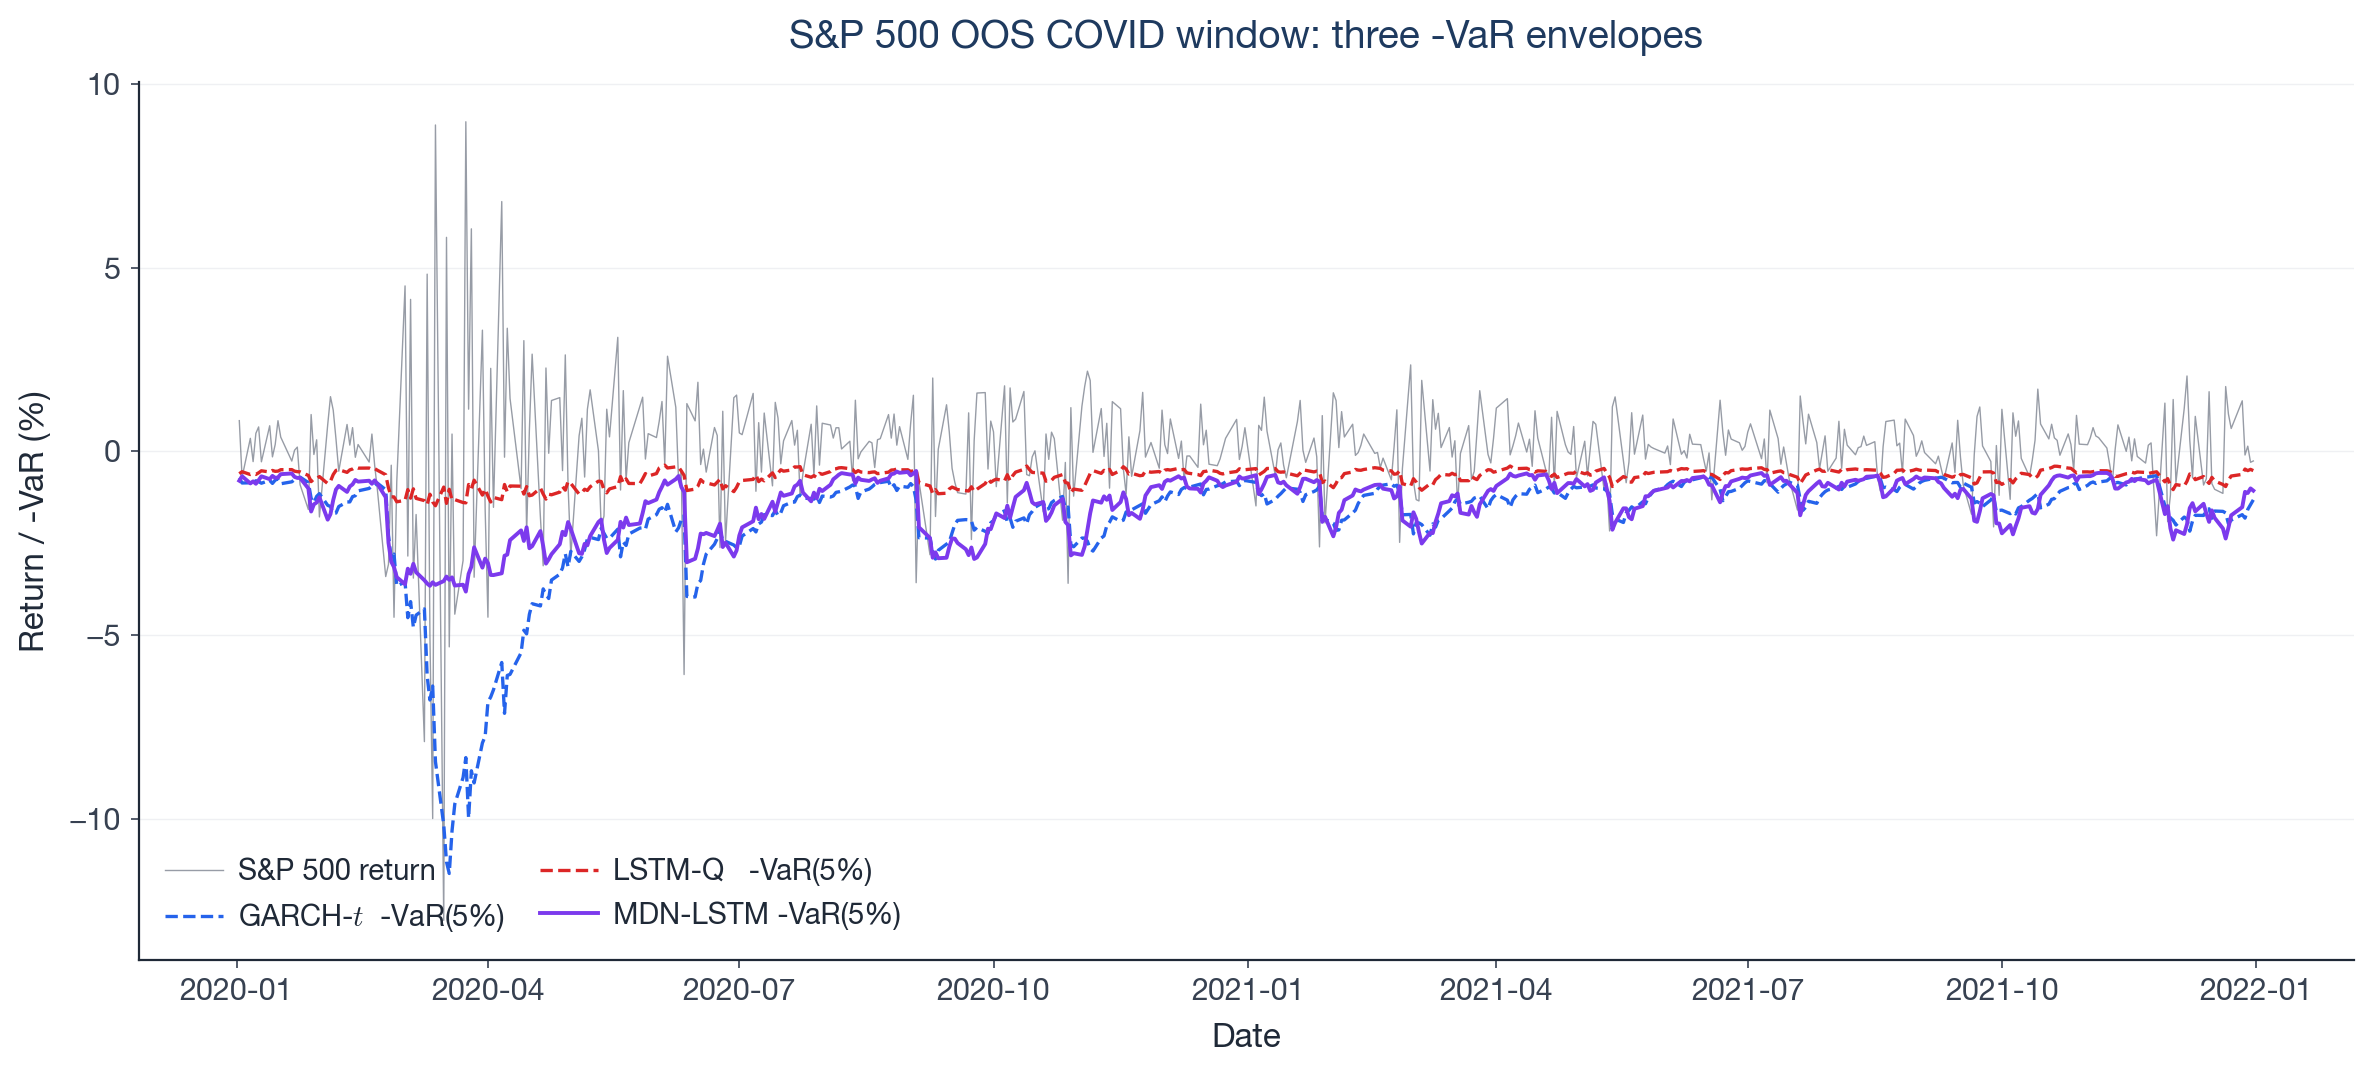
\includegraphics[width=0.98\textwidth]{../assets/figures/06_mdn_vs_lstm_vs_garch.png}
\caption{S\&P 500 daily returns over the COVID-19 OOS slice and the three
negative VaR envelopes ($\alpha = 0.05$): GARCH-$t$ scales with the realised
volatility regime, the LSTM-Quantile head holds approximately constant at
the level of the calm 2010--2019 in-sample window, and the MDN-LSTM sits
between the two.}
\label{fig:mdn-vs-lstm-garch}
\end{figure}

\subsection{Forecasting-model sensitivity: four GARCH variants}
\label{sec:res-multi-model}

The replication picks AR(1)-GARCH(1,1)-$t$ because that is the
forecasting model in \citet{du_escanciano_2017}. The choice is not
innocuous: four nearby specifications differ in their backtest
verdict on the same COVID-19 OOS window. Table~\ref{tab:multi-model}
runs the eleven base tests on the four combinations $(\text{vol},
\text{dist}) \in \{\text{GARCH}, \text{GJR}\} \times
\{t, \mathcal{N}\}$, sharing the AR(1) mean and the GARCH(1,1)
recursion and differing only in the leverage term ($\mathrm{GJR}$ adds
$\gamma\,\one\{\varepsilon_{t-1} < 0\}\varepsilon_{t-1}^2$) and the
innovation distribution.

\begin{table}[ht]
\centering
\caption{Eleven backtests across four GARCH variants on the S\&P 500
COVID-19 OOS slice. Cells in bold are rejections at $5\%$. The last
two columns report the in-sample log-likelihood (2010-2019,
$T = 2{,}516$ days) and the rejection count at $5\%$. The
Acerbi--Szekely cells for the two Normal-innovation variants are
empty because the parametric simulator wired into the battery is
Student-$t$-only.}
\label{tab:multi-model}
\small
\setlength{\tabcolsep}{5pt}
\begin{tabular}{@{}l*{4}{S[table-format=1.4]}@{}}
\toprule
\textbf{Test} & {\textbf{GJR-$t$}} & {\textbf{GARCH-$t$}} & {\textbf{GJR-$\mathcal{N}$}} & {\textbf{GARCH-$\mathcal{N}$}} \\
\midrule
$U_{ES}$              & \bfseries 0.0111 & \bfseries 0.0199 & 0.0600           & \bfseries 0.0418 \\
$C_{ES}(5)$           & 0.2366           & \bfseries 0.0164 & 0.4153           & \bfseries 0.0385 \\
$U_{VaR}$             & \bfseries 0.0159 & \bfseries 0.0025 & \bfseries 0.0452 & \bfseries 0.0273 \\
$C_{VaR}(5)$          & 0.9899           & \bfseries 0.0045 & 0.5274           & \bfseries 0.0117 \\
$Z_1$                 & \bfseries 0.0140 & 0.1070           & {---}            & {---}            \\
$Z_2$                 & \bfseries 0.0000 & \bfseries 0.0006 & {---}            & {---}            \\
$\mathrm{McNeil}\text{--}\mathrm{Frey}$ & 0.0848 & 0.1698 & \bfseries 0.0132 & \bfseries 0.0010 \\
$\mathrm{Kupiec}_{POF}$         & \bfseries 0.0237 & \bfseries 0.0052 & 0.0579           & \bfseries 0.0375 \\
$\mathrm{Christoffersen}_{CCI}$ & 0.8575           & 0.2998           & 0.7061           & 0.7810           \\
$\mathrm{Christoffersen}_{CC}$  & 0.0763           & \bfseries 0.0117 & 0.1542           & 0.1106           \\
$\mathrm{KLM}_{\text{mult}}(4)$ & 0.0838           & \bfseries 0.0088 & \bfseries 0.0284 & \bfseries 0.0017 \\
\midrule
\textbf{Rejections / tested}    & {$5/11$}         & {$8/11$}         & {$3/9$}          & {$7/9$}          \\
\textbf{Log-likelihood (IS)}    & {$-2860.23$}     & {$-2915.35$}     & {$-2936.60$}     & {$-3002.10$}     \\
\bottomrule
\end{tabular}
\end{table}

In-sample, the four variants rank cleanly: $\mathrm{GJR}\text{-}t$
($-2860.23$) dominates $\mathrm{GARCH}\text{-}t$ ($-2915.35$) by
$55$ log-points; the Student-$t$ variants beat the Normal variants
by a much larger margin. The order survives OOS: the rejection count
drops from $8/11$ for $\mathrm{GARCH}\text{-}t$ to $5/11$ for
$\mathrm{GJR}\text{-}t$ on the same data. The asymmetric variance
recursion routes more variance toward days following negative shocks,
which is exactly the clustering pattern $C_{ES}(m)$ and $C_{VaR}(m)$
detect; with $\gamma > 0$ the conditional Box-Pierce p-values move
from $0.0164$ to $0.2366$ and from $0.0045$ to $0.9899$
respectively. The Acerbi--Szekely $Z_1$ test inverts: $\mathrm{GJR}\text{-}t$
rejects ($p = 0.014$) where $\mathrm{GARCH}\text{-}t$ does not
($p = 0.107$), because the leverage term predicts a smaller ES on
the violation days and the realised severities exceed it.

The two Normal-innovation variants lose the AS p-values for the
reason given in the table caption; their remaining tests show that
$\mathrm{KLM}_{\text{mult}}(4)$ rejects in both cases ($p < 0.05$),
which is the multinomial substitute for the missing Acerbi--Szekely
signal. The Normal-innovation variants are dominated in
log-likelihood and miss the AS block, so they are not competitive
forecasting choices for an OOS slice that contains a fat-tail event.
Figure~\ref{fig:multi-model-heatmap} renders the eleven-by-four p-value
grid; variants are ordered by in-sample log-likelihood.

\begin{figure}[ht]
\centering
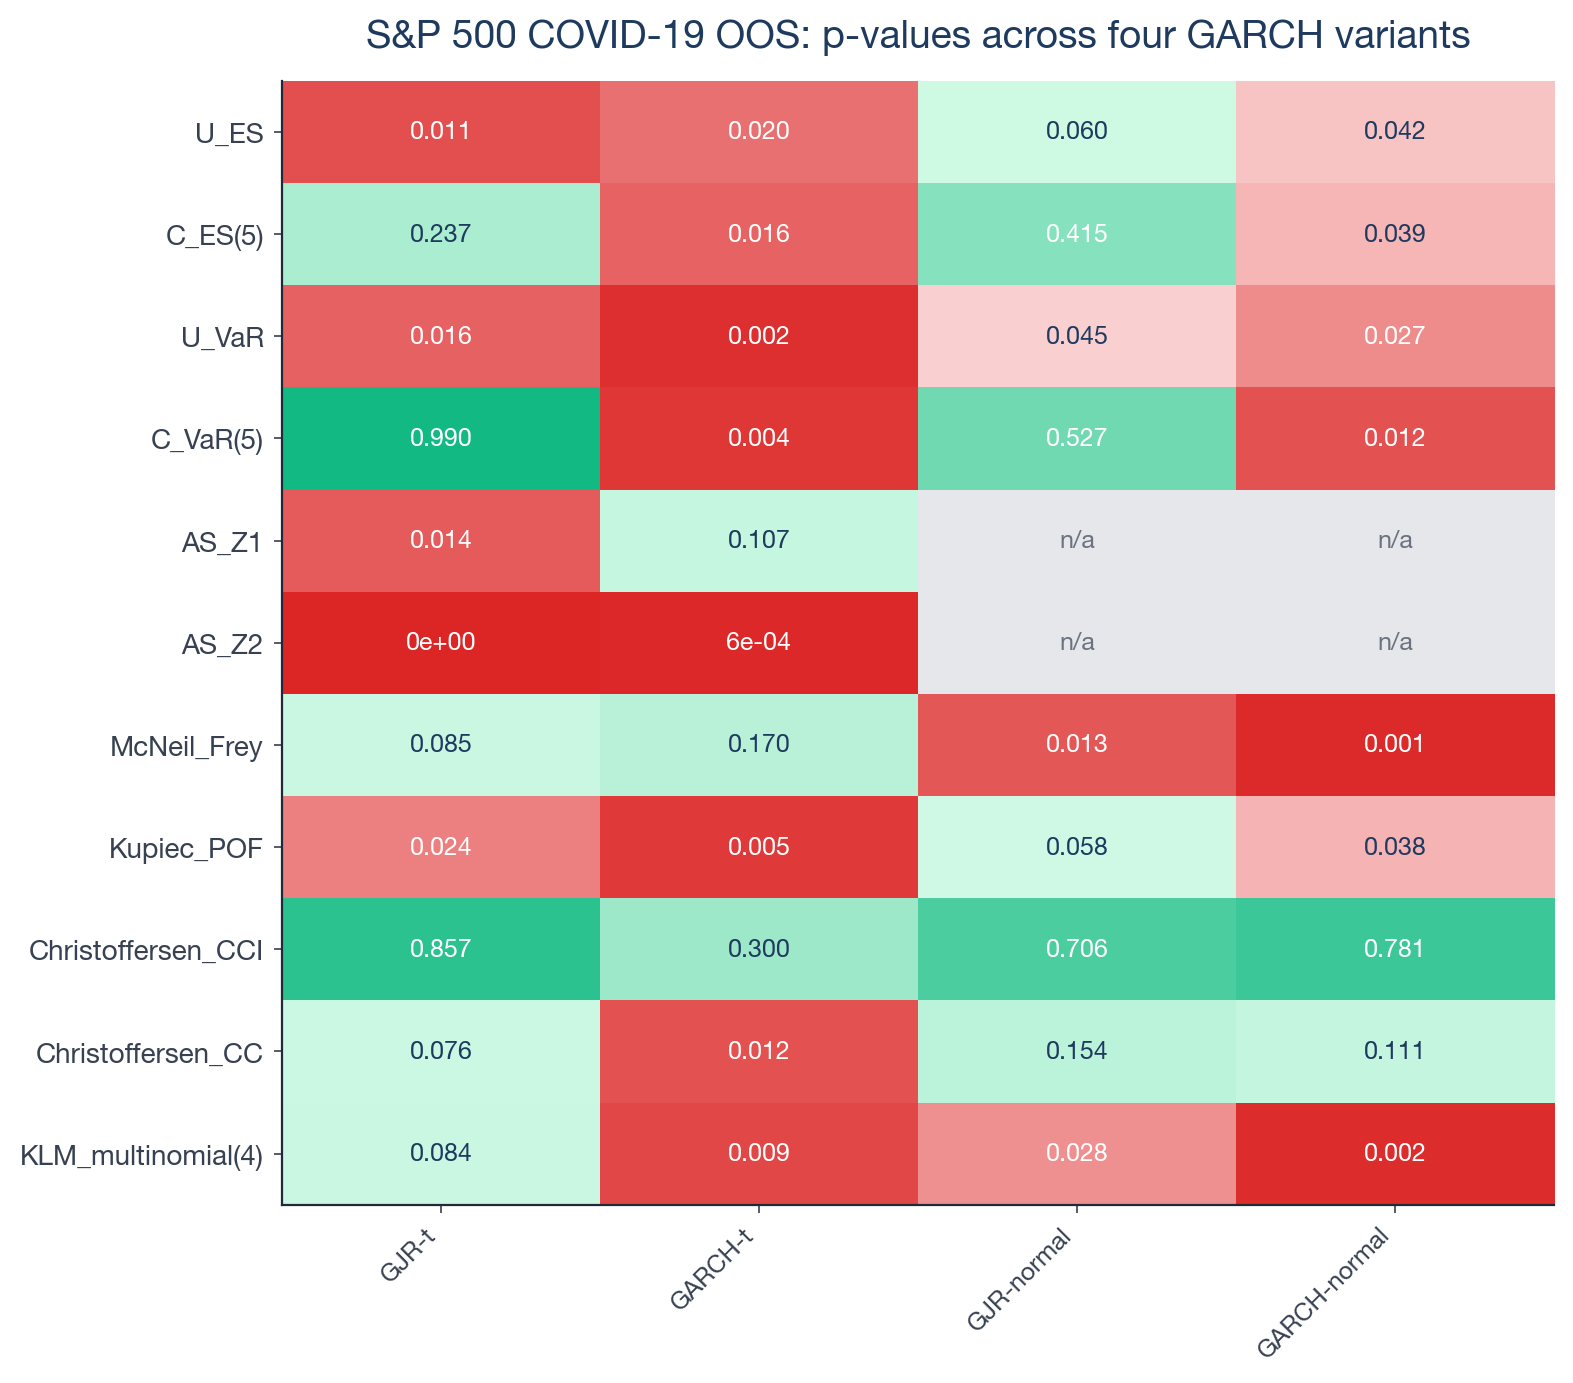
\includegraphics[width=0.95\textwidth]{../assets/figures/05_multi_model_heatmap.png}
\caption{P-value heatmap across (test) $\times$ (variant) cells on the S\&P 500
COVID-19 OOS slice. Cells with $p < 0.05$ are shaded red, cells failing to
reject are shaded green; the intensity tracks distance from the threshold.
Variants are ordered left-to-right by in-sample log-likelihood (best first):
$\mathrm{GJR}\text{-}t$, $\mathrm{GARCH}\text{-}t$,
$\mathrm{GJR}\text{-}\mathcal{N}$, $\mathrm{GARCH}\text{-}\mathcal{N}$.}
\label{fig:multi-model-heatmap}
\end{figure}

%% =====================================================================
\section{Discussion}
\label{sec:discussion}

The empirical results in Section~\ref{sec:results} converge on three
findings that have operational implications for ES backtesting.

\paragraph{Eleven tests give eleven answers.} On the same out-of-sample
slice, the unconditional and conditional Du--Escanciano statistics,
the Kupiec proportion-of-failures, the Christoffersen decomposition,
the Kratz--Lok--McNeil multinomial test, the Acerbi--Szekely $Z_1$
and $Z_2$, and the McNeil--Frey bootstrap occupy different regions of
the p-value space. On the S\&P 500 GFC window the tests split nine
to four; on the COVID window ten to three; the three tests that fail
to reject on both windows ($\mathrm{Christoffersen}_{CCI}$, $Z_1$,
McNeil--Frey) overlap. On the multi-asset grid the pattern is
sharper: the marginal-coverage block reaches $19$--$20$ of $20$
non-SVB cells, the conditional Box--Pierce block reaches $7$--$9$,
$\mathrm{Christoffersen}_{CCI}$ reaches $2$. The choice of test is
therefore not a sensitivity check on the result; it is a choice of
which channel of mis-specification the test is designed to see. The
unconditional block sees the violation count, $C_{ES}(m)$ sees
clustering in the cumulative severity, $Z_2$ sees the joint
frequency-and-magnitude tail behaviour, $Z_1$ and McNeil--Frey see
the severity conditional on a violation.

\paragraph{The Christoffersen decomposition is more informative than
the joint test.} The $\mathrm{LR}_{CC} = \mathrm{LR}_{POF} +
\mathrm{LR}_{IND}$ decomposition is exact. The empirical results
assign almost the entire signal to $\mathrm{LR}_{POF}$, which is also
the simpler test. A practitioner running only $\mathrm{LR}_{CC}$
would observe a rejection without learning whether the failure
comes from violation count or from clustering; the decomposition
recovers that information at no additional computational cost. The
case for reporting $(\mathrm{LR}_{POF}, \mathrm{LR}_{IND})$ rather
than $\mathrm{LR}_{CC}$ is thus diagnostic, not statistical.

\paragraph{$Z_2$ dominates $Z_1$ under leverage and on real crises.}
The Monte Carlo study shows that $Z_2$'s net power under strong
asymmetric leverage at $n = 1{,}000$ is $+9$~pp while $Z_1$'s is
$0$~pp. The same hierarchy holds on real data: across the twenty
non-SVB cells in the grid, $Z_2$ rejects in $19$, $Z_1$ in $5$.
The two statistics are sometimes presented as alternatives among the
``Acerbi--Szekely tests''; the empirical evidence here suggests
treating them as different tests. A practitioner who wants a single
ES-specific check that responds to leverage would pick $Z_2$.

\paragraph{Marginal-coverage tests over-reject at moderate $n$.} Under
correctly-specified DGP the empirical size at $n = 1{,}000$ is $0.16$
for $U_{ES}$ and McNeil--Frey, $0.14$ for $U_{VaR}$ and $Z_2$, $0.13$
for $\mathrm{Kupiec}_{POF}$ and $\mathrm{KLM}_{\text{mult}}(4)$, and
$0.12$ for $Z_1$ and $\mathrm{Christoffersen}_{CC}$. The asymptotic
$\chi^2$ and $\mathcal{N}(0,1)$ distributions are reached only at
substantially larger $n$. Calibration of operational backtest
thresholds should account for this size distortion; quoting a $5\%$
nominal threshold for $U_{ES}$ at $n = 1{,}000$ overstates the
type-I rate by a factor of roughly $3.2$.

\paragraph{Neural baselines do not generalise across volatility
regimes.} The LSTM-Quantile head trained on $2010$--$2019$
under-calls COVID-19 VaR by a factor of $2.6$. Both models reject
the Kupiec test, but the LSTM's rejection is twenty times stronger
than the GARCH's. The architecture is not a substitute for an
explicit volatility-clustering model when the OOS slice contains a
regime that the training data does not.

\paragraph{The MDN-LSTM fixes the architectural gap, not the
regime-shift one.} Replacing the two-output head with three heads
that parameterise the Student-$t$ distribution supplies the PIT,
the analytic VaR and ES, and the parametric simulator the
LSTM-Quantile lacks. Eleven of the thirteen statistics now apply
on the neural baseline. The MDN-LSTM also under-calls COVID-19 VaR
($1.45\%$ versus GARCH-$t$'s $1.83\%$), but at a factor of $1.3$
rather than $2.6$ -- the parametric output lets the neural network
learn a fat-tailed conditional distribution from the in-sample
window. The remaining gap is a training-data issue, not an
architectural one.

\paragraph{The GARCH-variant choice is part of the backtest.} Holding
the OOS slice and the test battery fixed, swapping the symmetric
GARCH(1,1) for the asymmetric GJR(1,1,1) flips five of the eleven
verdicts (Table~\ref{tab:multi-model}): the conditional Box-Pierce
statistics on cumulative violations relax to non-rejection, the
$\mathrm{Christoffersen}_{CC}$ statistic relaxes, the multinomial
test relaxes. The Acerbi--Szekely $Z_1$ inverts in the opposite
direction. The empirical evidence says that ``which test'' and
``which model'' are coupled choices that need to be reported
together; the practice of fixing the forecasting model and reporting
backtest results as a model-validation statement on its own is a
half-question.

%% =====================================================================
\section{Conclusion}
\label{sec:conclusion}

Expected shortfall as a regulatory risk measure has clean theoretical
foundations and a fragmented backtesting literature. This paper
implements eleven of the leading ES and VaR backtests in a single
unified battery and shows that the choice of a single test materially
shapes the verdict. On the S\&P 500 the eleven tests disagree on
three of the thirteen statistics on every crisis window; on a grid
of five indices and five crises they disagree on twenty p-values out
of twenty per non-trivial test. The Monte Carlo size-and-power study
quantifies the under- and over-rejection of each test at finite
sample sizes and shows that $Z_2$ dominates $Z_1$ by a wide margin
against asymmetric leverage. A four-variant sensitivity check
isolates the contribution of the GARCH choice: switching from
symmetric GARCH to asymmetric GJR flips five of the eleven verdicts
on the same OOS data. A mixture-density LSTM extends the classical
neural baseline so it can run on the full battery, cutting the COVID
under-call from a factor of $2.6$ to a factor of $1.3$. The
operational takeaway is that ES should not be backtested by a single
statistic, and that the choice of forecasting model is part of the
backtest rather than a separable input.

The implementation is a self-contained Python package
(\package{esback}) released under the MIT licence; the architecture
and the recipe to reproduce every number in this paper are documented
in Appendices~\ref{app:architecture} and~\ref{app:reproducibility}.

\bibliographystyle{plainnat}
\bibliography{refs}

%% =====================================================================
\appendix
\section{Software architecture}
\label{app:architecture}

The implementation is organised under \code{src/esback/}:
\begin{itemize}
  \item \code{config.py}, \code{\_logging.py}: project-wide constants
    (random seed, paths) and logging.
  \item \code{data/cache.py}, \code{data/loaders.py}: parquet cache
    around the \package{yfinance} downloader, with a frozen reference
    series under \code{tests/data/}.
  \item \code{models/ar1\_garch\_t.py}: baseline
    AR(1)-GARCH(1,1)-$t$ fit and the shared
    \code{\_garch\_recursion} helper used by every variant.
  \item \code{models/garch\_variants.py}: GJR-GARCH and Gaussian
    innovation variants routing through the shared recursion.
  \item \code{models/dl/}: the LSTM-Quantile head and its pinball $+$
    FZ0 loss functions, on top of PyTorch.
  \item \code{pit.py}, \code{risk\_measures.py}: PIT residual
    transforms and closed-form $\VaR_t$, $\ES_t$ for the standardised
    Student-$t$ and Normal innovations.
  \item \code{backtests/du\_escanciano.py}: the four basic and the
    two robust Du--Escanciano statistics.
  \item \code{backtests/var\_baselines.py}: Kupiec POF,
    Christoffersen CCI and CC, Kratz--Lok--McNeil multinomial.
  \item \code{backtests/es\_baselines.py}: Acerbi--Szekely $Z_1$
    and $Z_2$ with their parametric simulator; the McNeil--Frey
    bootstrap.
  \item \code{backtests/battery.py}: unified
    \code{run\_full\_battery} entry point.
  \item \code{pipeline.py}, \code{multi\_asset.py},
    \code{simulation/}: single-period, multi-asset and Monte Carlo
    orchestration.
  \item \code{viz/style.py}, \code{viz/figures.py}: a single palette
    and \code{apply\_rcparams} helper plus thirteen figure builders.
  \item \code{cli.py}: \code{esback replicate} and
    \code{esback multi-asset} entry points, wired through
    \package{typer}.
\end{itemize}
The unified battery is exposed as
\code{run\_full\_battery(\dots)}~$\to$~\code{dict[str, BacktestResult]}.
Every \code{BacktestResult} carries the test name, the statistic,
the p-value, the alpha at which the test was run, an asymptotic-null
reference and a free-form \code{extra} dictionary for diagnostic
quantities.

\section{Reproducibility}
\label{app:reproducibility}

The package supports a deterministic end-to-end re-run on Python
$\geq 3.11$. The recommended setup is
\begin{verbatim}
pip install -e ".[dev]"
pytest
\end{verbatim}
followed by the two command-line entry points
\begin{verbatim}
esback replicate    -c configs/replication_du_escanciano.yaml
esback multi-asset  -c configs/multi_asset_crisis.yaml
\end{verbatim}
which run in $\sim$2 seconds and $\sim$3 minutes on Apple Silicon
respectively. The S\&P 500 returns series is pinned to a parquet file
under \code{tests/data/}; the regression test suite under
\code{tests/integration/test\_regression.py} asserts that PIT
residuals, VaR and ES paths, and every backtest p-value match the
committed reference outputs to $10^{-10}$ on path quantities and to
$10^{-12}$ on p-values. The Monte Carlo study results are cached to
\code{results/power\_study/results.parquet}; a refresh is triggered
by deleting that file.

The package is style- and type-checked under \package{ruff} and
\package{mypy}; the unit and integration suites cover $181$ tests
that run in under ten seconds. The notebooks under
\code{notebooks/} are executable from a clean checkout via
\code{jupyter nbconvert --to notebook --execute --inplace}; the six
notebooks regenerate the ten figures bundled under
\code{assets/figures/}.

\end{document}
